\section{Case study: Berry, Levinsohn and Pakes (1995), U.S. automobiles}\label{sec:08-blp95}

\citet{BerryLevinsohnPakes1995}, henceforth BLP, turned the random coefficients logit into a working
tool for industrial organization. They estimate demand and marginal cost for essentially every car
model sold in the United States from 1971 to 1990. They use only product-level data on prices,
quantities and characteristics, together with the distribution of household income. The estimates
come from a model in which consumers choose one car or none and multi-product firms set prices in a
Nash equilibrium.

The general model, its computation and its identification occupy
\cref{sec:08-model,sec:08-substitution,sec:08-simulation,sec:08-inversion,sec:08-gmm,sec:08-instruments,sec:08-supply}.
This section applies that machinery to the paper itself. We follow the order used for every deep case
study in this book. We take up the question, the setting, the data, the model, and the estimator with
its identification. Then come the results, robustness, interpretation, critiques and contribution. We
reproduce the
paper's Tables III, IV, V, VII, VIII and IX in full, Table I in condensed form, and an excerpt of
Table VI. Several derived quantities in this section are our own calculations from the published
tables, and we say so each time.

\subsection{The question and why it matters}\label{sec:08-blp95-question}

The paper asks how to recover demand and cost parameters for a whole differentiated-products industry
when only market-level data are available. The answers must be consistent with an oligopoly
equilibrium. On the demand side BLP want own- and cross-price elasticities for every model, and
elasticities of demand with respect to attributes such as fuel efficiency. On the cost side they want
marginal cost as a function of product characteristics.

These objects are inputs to many policy questions. BLP list trade policy (import restrictions),
merger policy, environmental policy (gas-guzzler and carbon taxes, emission standards and fuel
economy standards) and the construction of price indices (Section 8.1 of the paper). The automobile
market was large, with sales above \$150 billion in 1989 (p.~843). It was also at the center of trade
and environmental debates.

The obvious alternative is a demand system written directly in product space. A constant-elasticity
system for 100 products has 10,000 own- and cross-price elasticities (p.~842). Researchers therefore
aggregate products into groups. BLP point out that a grouping that suits one question rarely suits
another. Aggregating all foreign and all domestic cars may serve a tariff study, but it is useless for
domestic competition or pollution taxes. Product-space systems also cannot predict demand for new
goods, and they make it hard to use information on the distribution of consumers.

BLP work in characteristics space, following \citet{Lancaster1971} and \citet{McFadden1974}. They
identify two problems with the discrete-choice models available at the time. The first is the
functional form of utility, which in logit-type models forces implausible substitution patterns. The
second is the correlation between price and product characteristics that consumers see and the
econometrician does not. BLP call this the differentiated-products analog of the classical
simultaneity problem. They solve the aggregation problem by simulation, as in \citet{Pakes1986}. They
solve the simultaneity problem by inverting the share equations, as in \citet{Berry1994}.

\subsection{Setting and earlier approaches}\label{sec:08-blp95-setting}

Early work treated cars as a homogeneous product and estimated aggregate demand \citep{Suits1958}.
\citet{Griliches1971} introduced hedonic price regressions for cars, which work at the level of the
individual model but do not model the production side. BLP call \citet{Bresnahan1987} perhaps the first
attempt to model and estimate demand and oligopoly pricing jointly (p.~844). He used a vertical differentiation model with a
uniform density of consumers along the quality line (\cref{ch:discrete}).
\citet{FeenstraLevinsohn1995} allowed several dimensions of differentiation but kept the uniform
density. \citet{Manski1983} studied demand and a perfectly competitive supply side for the Israeli car
market.

Micro-data studies of car demand had alternatives to BLP's solutions. They could interact consumer
and product characteristics, or use nested logit, which BLP note is a restricted random coefficients
model on group dummies (p.~851). Nested logit requires a priori knowledge of the order and content of
the nests. Product-specific constants, which would absorb unobserved quality, are hard to estimate with
micro data. There are on average more than 100 products per year in BLP's sample. The Consumer
Expenditure Survey records only about 500 new-car purchases per year (p.~852). Even with product
dummies, one still has to separate the effects of price, observed characteristics and unobserved
quality, which requires the kind of instrumental-variable assumptions BLP make.

The vertical model restricts substitution severely. A product has nonzero cross-price elasticities only
with its two neighbors on the price ladder. BLP give an example with a \$24,998 station wagon, a
\$24,999 sports car and a \$25,000 station wagon (p.~852). The vertical model makes the two wagons
non-substitutes and the sports car a substitute for both. The logit model fails in the opposite way.
If a cheap Yugo and an expensive Mercedes have the same share, a rise in the BMW's price must raise
both of their sales by the same amount (p.~847). Two products with equal shares must also have equal
own-price derivatives, and hence equal markups under single-product pricing
(\cref{sec:08-substitution}).

Finally, BLP stress the structural error $\xi_{jt}$. Without it, only sampling error separates the
model's predicted shares from the data. With aggregate samples of millions of households, a
chi-square test of the model's restrictions on the multinomial shares rejects with probability close
to one (p.~850). The unobserved characteristic plays the role of the demand disturbance in
homogeneous-goods markets. Because firms know it when they set prices, prices are correlated with it.

\subsection{Data}\label{sec:08-blp95-data}

The unit of observation is a car model in a year, and a market is the national market in a year.
Product characteristics come from annual issues of the \emph{Automotive News Market Data Book},
combined with a similar data set from Ernst Berndt (p.~868). The sample covers essentially all models
sold from 1971 to 1990. Only ``exotic'' models with tiny shares, such as Ferrari and Rolls Royce, are
excluded. The panel is unbalanced because models enter and exit. It has 2,217 model-years.

BLP need a rule that links model-years into models, because their standard errors allow correlation
within a model over time. Two observations in adjacent years are the same model if they have the same
name and their horsepower, width, length and wheelbase each change by at most ten percent. With this
rule the 2,217 model-years represent 997 distinct models (p.~869).

The variables are as follows.
\begin{itemize}
\item \emph{Price} is the list retail price of the base model, in thousands of 1983 dollars (deflated
  by the CPI). BLP would prefer transaction prices but could not find them.
\item \emph{Quantity} is U.S. sales by nameplate, in thousands. Fleet sales are not observed, so fleet
  buyers are treated as agents of households (footnote 23).
\item \emph{HPWT} is horsepower divided by weight, in horsepower per 10 pounds.
\item \emph{Air} equals one if air conditioning is standard equipment.
\item \emph{MP\$} (miles per dollar) is the EPA miles-per-gallon rating divided by the real price of
  unleaded gasoline. It measures the cost of driving and enters utility. The production cost of fuel
  efficiency is captured instead by \emph{MPG}, which enters the cost function.
\item \emph{Size} is length times width.
\item \emph{Reliability} is the Consumer Reports rating from 1 to 5, available for part of the sample
  and rescaled every year (footnote 24). It appears only in one robustness check.
\end{itemize}
The market size $M_t$ is the number of U.S. households in year $t$, from the \emph{Statistical
Abstract}. The parameters of the household income distribution come from the March Current Population
Survey (CPS) for each year. Divisions of one parent company form one firm, so Buick, Cadillac,
Chevrolet, Oldsmobile and Pontiac all belong to General Motors. There are 22 firms (footnote 29). Each
model is assigned the country of its producing firm.

\begin{table}[htbp]
\centering
\caption{Descriptive statistics of the BLP (1995) data, selected years (condensed from their Table I)}
\label{tab:08-blp-desc}
\footnotesize
\setlength{\tabcolsep}{3.6pt}
\begin{tabular}{@{}lrrrrrrrrrrr@{}}
\toprule
Year & Models & Quantity & Price & Domestic & Japan & Europe & HPWT & Size & Air & MPG & MP\$ \\
\midrule
1971 & 92  & 86.892  & 7.868  & 0.866 & 0.057 & 0.077 & 0.490 & 1.496 & 0.000 & 1.662 & 1.850 \\
1973 & 86  & 92.785  & 7.535  & 0.932 & 0.040 & 0.028 & 0.364 & 1.529 & 0.022 & 1.589 & 1.819 \\
1974 & 72  & 105.119 & 7.506  & 0.887 & 0.050 & 0.064 & 0.347 & 1.510 & 0.026 & 1.568 & 1.453 \\
1975 & 93  & 84.775  & 7.821  & 0.853 & 0.083 & 0.064 & 0.337 & 1.479 & 0.054 & 1.584 & 1.503 \\
1980 & 103 & 71.567  & 7.718  & 0.773 & 0.191 & 0.036 & 0.350 & 1.296 & 0.078 & 2.215 & 1.466 \\
1985 & 136 & 78.143  & 8.938  & 0.761 & 0.191 & 0.048 & 0.372 & 1.265 & 0.140 & 2.261 & 2.024 \\
1988 & 150 & 67.078  & 10.069 & 0.717 & 0.237 & 0.045 & 0.396 & 1.251 & 0.237 & 2.334 & 2.919 \\
1990 & 131 & 66.377  & 10.337 & 0.682 & 0.276 & 0.043 & 0.419 & 1.270 & 0.308 & 2.270 & 2.852 \\
\midrule
All  & 2217 & 78.804 & 8.604  & 0.790 & 0.161 & 0.049 & 0.372 & 1.357 & 0.116 & 2.099 & 2.086 \\
\bottomrule
\end{tabular}

\smallskip
\begin{minipage}{0.97\linewidth}
\footnotesize
Notes: Source: \citet{BerryLevinsohnPakes1995}, Table I (p.~870), which reports all 20 years.
``Models'' is the number of models and ``Quantity'' is mean sales per model. The remaining nine columns
are sales-weighted means. Quantity is in thousands of cars and price in thousands of 1983 dollars. HPWT
is in horsepower per 10 pounds, MPG in tens of miles per gallon and MP\$ in tens of miles per 1983 dollar
of gasoline. Domestic, Japan and Europe are
dummies for the location of the producing firm's headquarters.
\end{minipage}
\end{table}

\Cref{tab:08-blp-desc} shows the main trends. The number of models rose from a low of 72 in 1974 to a
high of 150 in 1988, while sales per model trended down. The sales-weighted list price stayed between
about \$7,500 and \$8,000 during the 1970s. It then rose from \$7,718 in 1980 to \$10,337 in 1990, about a
third.\footnote{The text of \citet[p.~870]{BerryLevinsohnPakes1995} says that the real sales-weighted list price
``has risen almost 50 percent during the 1980's.'' Their Table I, which is already in 1983 dollars, implies an
increase of $\frac{10.337}{7.718} - 1 = 34$ percent from 1980 to 1990. Measured from the 1979 value of 7.599, the
increase is 36 percent. We follow the table.} The characteristics changed at the same time, so the price of a fixed bundle need not have
risen. HPWT fell in the early 1970s and then trended up, mostly because cars became lighter. Fuel cost
efficiency improved, from 18.50 miles per 1983 dollar of gasoline in 1971 to 28.52 in 1990. Air
conditioning was standard on no car at the start and on 30.8 percent at the end. The domestic share
fell from a 1973 high of 93.2 percent to 68.2 percent in 1990, while the Japanese share rose from 4.0 to
27.6 percent.

BLP's Table II reports quartiles of the continuous variables and names the models at each quartile.
The cheapest car is the 1990 Yugo at \$3,393 (1983 dollars). The median price is \$8,728 and the 75th
percentile is \$13,074. The most expensive car is a 1989 Porsche 911 Cabriolet at \$68,597. Sales range
from 49 cars to 577,313 cars (the 1971 Chevrolet Impala), with a median of 47,345. MPG ranges from 9
(1974 Cadillac Eldorado) to 53 (1989 Geo Metro). We use the price quartiles below to interpret the
logit results.

The data also pin down the size of the outside good. Total 1990 sales are about
$131\times 66.377\approx 8{,}695$ thousand cars (\cref{tab:08-blp-desc}). BLP describe the logit column
of their Table VII as $\frac{s_0}{1-s_j}$, and its entries lie between 90.458 and 90.883 percent.
Because $\frac{s_0}{1-s_j}$ exceeds $s_0$, the smallest entry bounds the outside share, $s_0 < 0.9046$.
The entries do not rise with the shares as the formula requires (the best-selling Accord has the
smallest entry), so we read them only as $s_0 \approx 0.90$. With $s_0$ near 0.90,
$M_{1990}=\frac{8.695}{1-s_0}$ is roughly 90 million households (our calculation). Most households do not buy a new car in a given year, so the outside good is large.

\subsection{The model}\label{sec:08-blp95-model}

\casehead{Utility}
BLP nest random coefficients in the Cobb-Douglas utility \eqref{eq:08-cobb-douglas} over the car's
characteristics and spending on other goods (their eq.~2.6). Its logarithm gives the inside and outside
utilities \eqref{eq:08-blp-inside} and \eqref{eq:08-blp-outside} (their eqs.~2.7a and 2.7b), which
\cref{sec:08-income} derived. BLP write $\bar\beta$ for our $\beta$. The taste shocks $\nu_{ik}$ have mean
zero and unit variance, so characteristic $k$ has marginal utility $\beta_k+\sigma_k\nu_{ik}$, with mean
$\beta_k$ and variance $\sigma_k^2$. The term $\sigma_0\nu_{i0}$ lets the outside option have more
idiosyncratic variance than the inside goods. BLP motivate it by unobserved differences in access to
public transport and in used-car holdings (p.~849).

BLP prefer this form to the plain random coefficients model
$u_{ij}=x_j\beta-\alpha p_j+\xi_j+\sum_k\sigma_kx_{jk}\nu_{ik}+\epsilon_{ij}$ (their eq.~2.5) for two
reasons (p.~848). They have outside information on the income distribution, and they have a
theoretical rationale for the form of the interaction between income and price. The Cobb-Douglas form
uses both.

\casehead{The estimated form}
The empirical model adds a year index $t$ and makes income random. Household income is lognormal,
$y_{it}=e^{m_t+\sigma_y\nu_{iy}}$, with year-specific mean $m_t$ and a common standard deviation
$\sigma_y$, both estimated from the CPS. The utility functions are \eqref{eq:08-blp-final-inside} and
\eqref{eq:08-blp-final-outside} (their eqs.~6.14a and 6.14b). The vector
$(\nu_{iy},\nu_{i0},\nu_{i1},\dots,\nu_{iK})$ is standard multivariate normal, independent of everything
else. BLP hold each simulated consumer's draws fixed over the 20 years of the panel. The idiosyncratic
shocks $\epsilon_{ijt}$ are \iid\ type-I extreme value. BLP did not estimate a separate $\sigma_y$ for each
year because those estimates were imprecise. They also tried drawing incomes directly from the CPS, which
gave imprecise simulators, especially in the upper tail (footnote 21).

The characteristics in utility are $x_{jt}=(1,\mathit{HPWT}_{jt},\mathit{Air}_{jt},
\mathit{MP\$}_{jt},\mathit{Size}_{jt})$, so $K=5$. Each has a mean $\beta_k$ and a standard deviation
$\sigma_k$. Price carries no separate random coefficient. Heterogeneity in price sensitivity comes
entirely from income, as we now show.

\casehead{Mean utility and individual deviations}
Choice probabilities depend only on utility differences, so we subtract \eqref{eq:08-blp-final-outside} from
\eqref{eq:08-blp-final-inside} and normalize $\xi_{0t}=0$. The deterministic part of the difference is
\begin{align*}
u_{ijt}-u_{i0t}-(\epsilon_{ijt}-\epsilon_{i0t})
 &=\alpha\big[\ln(y_{it}-p_{jt})-\ln y_{it}\big]+x_{jt}\beta+\xi_{jt}
   +\sum_k\sigma_kx_{jkt}\nu_{ik}-\sigma_0\nu_{i0}\\
 &=\underbrace{x_{jt}\beta+\xi_{jt}}_{\delta_{jt}}
   +\underbrace{\alpha\ln\Big(1-\frac{p_{jt}}{y_{it}}\Big)+\sum_k\sigma_kx_{jkt}\nu_{ik}
   -\sigma_0\nu_{i0}}_{\mu_{ijt}} .
\end{align*}
Three features of this decomposition matter for estimation. First, the mean utility
\begin{equation}\label{eq:08-blp-delta}
\delta_{jt}=x_{jt}\beta+\xi_{jt}
\end{equation}
contains no price term. Price enters only through $\mu_{ijt}$, so $\alpha$ is a nonlinear parameter.
In the chapter's notation $\theta_1=\beta$ and $\theta_2=(\alpha,\sigma_1,\dots,\sigma_5)$. Second, the
constant is the first characteristic ($x_{j1t}=1$), so the terms $\sigma_1\nu_{i1}-\sigma_0\nu_{i0}$
combine into one normal random variable with variance $\sigma_1^2+\sigma_0^2$. A random coefficient on
the inside-good constant and an extra shock on the outside good are therefore observationally
equivalent, and only the combined variance is identified. This is why BLP's footnote 6 describes
$\sigma_0\nu_{i0}$ as a random coefficient on the constant. The reported standard deviation on the
constant measures this combined dispersion. Third,
$\mu_{ijt}$ is defined only when $y_{it}>p_{jt}$. A simulated household whose income draw is below a
car's price cannot buy that car, and an implementation must remove the car from that household's
choice set.

\casehead{Market shares}
Conditional on $\nu_i$, integrating the extreme value shocks gives the logit form
\eqref{eq:08-individual-share} (their eq.~6.6). The market share \eqref{eq:08-share-integral} integrates over the
standard normal vector $\nu_i$, with income determined by $\nu_{iy}$ (their eq.~6.7). The inner integral has a
closed form and the outer one does not. BLP evaluate it by simulation (\cref{sec:08-simulation}).

\casehead{Price derivatives and elasticities}
Differentiating $\mu_{ijt}$ gives the price sensitivity of household $i$ for car $j$:
\begin{equation*}
\frac{\partial\mu_{ijt}}{\partial p_{jt}}=-\frac{\alpha}{y_{it}-p_{jt}} .
\end{equation*}
This sensitivity falls with income. It also rises with the car's own price, because a dollar is
worth more when less is left for other goods. A first-order expansion of the log for small
$\frac{p_{jt}}{y_{it}}$ gives
\begin{equation*}
\alpha\ln\Big(1-\frac{p_{jt}}{y_{it}}\Big)\approx-\alpha\,\frac{p_{jt}}{y_{it}},
\end{equation*}
so household $i$ behaves approximately as if its price coefficient were $\frac{\alpha}{y_{it}}$.
Applying the general derivative formulas of \cref{prop:08-derivs} with this price sensitivity gives
\begin{align}
\frac{\partial s_{jt}}{\partial p_{jt}}&=-\int\frac{\alpha}{y_{it}-p_{jt}}\,
  s_{ijt}(1-s_{ijt})\,\dd F(\nu_i),\label{eq:08-blp-dsown}\\
\frac{\partial s_{jt}}{\partial p_{qt}}&=\int\frac{\alpha}{y_{it}-p_{qt}}\,s_{ijt}s_{iqt}\,
  \dd F(\nu_i),\qquad q\neq j\label{eq:08-blp-dscross}
\end{align}
(their eqs.~6.9a and 6.9b). The derivative of the outside share is
$\frac{\partial s_{0t}}{\partial p_{qt}}=\int\frac{\alpha}{y_{it}-p_{qt}}s_{i0t}s_{iqt}\,\dd F(\nu_i)$.

BLP report \emph{semi-elasticities}, which we denote
\begin{equation}\label{eq:08-blp-semi}
e_{jq}\equiv\frac{100}{s_j}\,\frac{\partial s_j}{\partial p_q},
\end{equation}
with prices in thousands of dollars. The entry $e_{jq}$ is the percentage change in the share of $j$
when the price of $q$ rises by \$1,000. The elasticity follows by multiplying by
$\frac{p_q}{100}$, so the own-price elasticity, written as a positive number, is
$\varepsilon_j=-\frac{p_j}{100}\,e_{jj}$. The logit benchmark has $e_{jj}=-100\,\alpha(1-s_j)$ and
$e_{jq}=100\,\alpha s_q$.

\casehead{Costs and pricing}
Firm $f$ produces the set $\mathcal{J}_f$ of models. Marginal cost is constant in output and log-linear
in observed cost characteristics $w_j$ and an unobserved cost shock $\omega_j$:
\begin{equation}\label{eq:08-blp-mc}
\ln mc_j=w_j\gamma+\omega_j
\end{equation}
(their eq.~3.1). The cost characteristics are a constant, $\ln\mathit{HPWT}$, $\mathit{Air}$,
$\ln\mathit{MPG}$, $\ln\mathit{Size}$ and a time trend. MPG replaces MP\$ because the production cost
of fuel efficiency does not depend on the retail price of gasoline, at least in the short run. The
trend captures technical change and regulation. Logs of the continuous attributes make the cost
coefficients elasticities of marginal cost. BLP allow $\omega_j$ to be correlated with $\xi_j$, since
cars with more unobserved quality may cost more to build.

Firm $f$'s profit is \eqref{eq:08-profit} (their eq.~3.2), and each firm chooses its prices given rivals'
prices. An interior Nash equilibrium satisfies the first-order conditions \eqref{eq:08-foc} (their eq.~3.3).
\Cref{sec:08-supply-foc} showed that BLP's markup formula (their eqs.~3.4 and 3.5) is our
\eqref{eq:08-markup}, and that substituting it into \eqref{eq:08-blp-mc} gives the pricing equation
\eqref{eq:08-pricing-log} (their eq.~3.6). The markup depends on $\omega$ through the equilibrium prices, and on
$\xi$ directly. It therefore cannot be treated as exogenous in the pricing equation.

BLP assume that a Nash equilibrium exists with prices in the interior of the positive orthant
(footnote 12). The existence results of \citet{CaplinNalebuff1991} cover single-product firms and do
not extend easily to multi-product firms. BLP instead check existence numerically at their estimates.
None of the properties of the estimator requires a unique equilibrium. Without uniqueness, however, it
is not clear how to use the estimates for policy counterfactuals.

\subsection{Estimation and identification}\label{sec:08-blp95-estimation}

\casehead{Moment conditions}
Let $z_j=(x_j,w_j)$ collect the demand and cost characteristics of product $j$, and let
$z=(z_1,\dots,z_J)$ collect them for all products in the market. BLP's identifying assumption is
\begin{equation}\label{eq:08-blp-moments}
\E[\xi_j\mid z]=\E[\omega_j\mid z]=0
\end{equation}
(their eq.~4.1). Prices and quantities are excluded from the conditioning set because the model
determines them partly through $\xi$ and $\omega$. Characteristics and cost shifters are treated as
predetermined because the model does not explain how they are chosen.

BLP acknowledge that \eqref{eq:08-blp-moments} holds only if the true process that chooses
characteristics has special properties (p.~854). They mention an alternative for panel data. The
pair $(\xi,\omega)$ of a model could follow a first-order Markov process whose innovations are
independent of the model's initial characteristics. This assumption would also identify the model, but
it would demand much more of the data, so BLP start from \eqref{eq:08-blp-moments}.

\casehead{Why characteristics of other products are instruments}
Under \eqref{eq:08-blp-moments}, any function of $z$ is a valid instrument. The question is which
functions carry information. BLP's answer comes from oligopoly pricing (p.~855). Products that face
close substitutes have low markups, so the characteristics of rival products shift a product's price.
Nash markups respond differently to products of the same firm and to products of rivals. The
instruments should therefore distinguish the two. The demand for $j$ depends on the characteristics of
all products, so no characteristic is excluded from the demand of $j$ in the usual sense. What
identifies demand is the restriction that the utility of $j$ depends only on the characteristics of
$j$. The number of utility parameters then grows with the number of characteristics, and not with the
number of products.

\casehead{The instrument vector}
The efficient instruments under conditional moment restrictions are infeasible here
(\cref{sec:08-optiv}). BLP instead use the first-order terms \eqref{eq:08-blp-iv} of a partially
exchangeable basis (their eq.~5.8). These are the own characteristic, its sum over the firm's other products
and its sum over rival products. \Cref{sec:08-optiv} derives this basis from the exchangeability of a
unique Nash equilibrium \citep{Pakes1994}. The two sums vary across products because they exclude different
own products, because firms offer different sets of products, and because the set of products changes over
time. The constant is one of the characteristics, so the numbers of own-firm and rival products are
instruments too.

Higher-order basis functions were nearly collinear with the first-order terms, and even the first-order
terms were nearly of reduced rank. For the demand error BLP use the three terms of
\eqref{eq:08-blp-iv} for each of the five demand characteristics, giving 15 instruments. MPG and the
trend enter cost and not demand, so they are excluded from demand. Adding them to the demand list caused
numerical problems through near collinearity, and BLP left them out. For the cost error BLP use the three terms for each of the six cost characteristics,
plus MP\$, giving 19 instruments. The estimator therefore uses $15+19=34$ moment conditions (p.~862).
There are 17 parameters: five means $\beta$, five standard deviations $\sigma$, the income coefficient
$\alpha$ and six cost parameters $\gamma$. Hence there are 17 overidentifying restrictions.

BLP enter the basis functions directly as GMM instruments, instead of first projecting the optimal
instruments on them as \citet{Newey1990} suggests (\cref{sec:08-optiv}).

\casehead{Clustering by model}
Disturbances of the same model in different years are likely to be more similar than those of
different models. BLP therefore treat the sum of a model's moments over the years it is sold as one
draw from an exchangeable population of models. Let $z^d_{mt}$ and $z^s_{mt}$ be the 15 demand and 19
cost instruments of model $m$ in year $t$, and let $\mathcal{T}_m$ be the years in which $m$ is sold.
The moment contribution of model $m$ is
\begin{equation}\label{eq:08-blp-gm}
g_m(\theta)=\sum_{t\in\mathcal{T}_m}\begin{pmatrix} z^{d\T}_{mt}\,\xi_{mt}(\theta)\\
z^{s\T}_{mt}\,\omega_{mt}(\theta)\end{pmatrix}\in\R^{34}.
\end{equation}
BLP write this as $\sum_t[f_{mt}(z)^{\T}\otimes I_2](\xi_{mt},\omega_{mt})^{\T}$, with the
instrument blocks restricted as described above. The estimator minimizes
\begin{equation}\label{eq:08-blp-obj}
Q(\theta)=\bar g(\theta)^{\T}\,W\,\bar g(\theta),\qquad
\bar g(\theta)=\frac{1}{997}\sum_{m=1}^{997}g_m(\theta),
\end{equation}
with $W$ a consistent estimate of the inverse covariance matrix of $g_m$. The resulting standard errors
allow arbitrary correlation across years within a model and arbitrary heteroskedasticity across
models. BLP note that this is probably not the most efficient way to use the panel.

\casehead{Computing the objective}
Each evaluation of the moments takes four steps for a given $\theta$ (p.~863).
\begin{enumerate}
\item Simulate the market shares $s_{jt}(\delta_t;\theta_2)$ implied by the model.
\item Solve for the mean utilities $\delta_t$ that equate simulated and observed shares, and set
  $\xi_{jt}=\delta_{jt}-x_{jt}\beta$.
\item Compute the markups $b_{jt}$ from the simulated share derivatives and set
  $\omega_{jt}=\ln(p_{jt}-b_{jt})-w_{jt}\gamma$.
\item Interact $\xi$ and $\omega$ with the instruments to form \eqref{eq:08-blp-gm}.
\end{enumerate}
The logit benchmark puts price in the mean utility, $\delta_{jt}=x_{jt}\beta-\alpha p_{jt}+\xi_{jt}$, and
sets $\mu_{ijt}=0$. Every step is then analytic. Shares are
$s_{jt}=\frac{e^{\delta_{jt}}}{1+\sum_qe^{\delta_{qt}}}$, the inversion is
$\delta_{jt}=\ln s_{jt}-\ln s_{0t}$, and the demand error is
$\xi_{jt}=\ln s_{jt}-\ln s_{0t}-x_{jt}\beta+\alpha p_{jt}$ (their eqs.~6.3 to 6.5). In the full model
step~2 uses the contraction
\begin{equation*}
\delta_{jt}^{h+1}=\delta_{jt}^{h}+\ln s^{\text{obs}}_{jt}-\ln s_{jt}\big(\delta_t^{h};\theta_2\big)
\end{equation*}
(their eq.~6.8), whose convergence BLP prove in their Appendix~I (\cref{thm:08-contraction}).

Step~1 uses the importance sampler \eqref{eq:08-blp-importance} of \cref{sec:08-importance} (their
eq.~6.13). BLP first obtain a preliminary estimate $\theta'$ with the plain smooth simulator. They then
accept population draws of $\nu$ with probability $\bar f(\nu;\theta')$, the probability that a household
with tastes $\nu$ buys some car, and reweight each accepted draw by $\frac{\bar s(\theta')}{\bar
f(\nu;\theta')}$. The sampler oversamples households likely to buy a car, which is where the integrand is
large. The same draws are used for every share, so the simulated shares sum to one, as the contraction
requires.

The first-order conditions of \eqref{eq:08-blp-obj} are linear in $\beta$ and $\gamma$ given
$(\alpha,\sigma)$. Both $\xi=\delta(\theta_2)-X\beta$ and $\omega=\ln(p-b(\theta_2))-W_c\gamma$ are linear
in the linear parameters, where $W_c$ stacks the $w_{jt}$. The markup depends only on $\theta_2$ because
it is computed from the inverted $\delta$ and the share derivatives. BLP concentrate out $\beta$ and
$\gamma$ as in \cref{prop:08-concentrate} and search over the six elements of $(\alpha,\sigma)$ with the
\citet{NelderMead1965} simplex method (p.~868).

\casehead{Standard errors}
The asymptotic variance is \eqref{eq:08-blp-avar}, the sandwich with the three variance pieces $V_1$
(product characteristics), $V_2$ (consumer sampling) and $V_3$ (simulation) derived in
\cref{sec:08-asymptotics}. With about 100 million U.S. households, $V_2$ is negligible and $V_3$ is not.
BLP estimate $V_3$ by redrawing the simulation draws. The correction raises the standard errors in their
Table IV by about 5 to 20 percent, except for one parameter whose standard error doubles (p.~859).

\casehead{What identifies the parameters}
Four sources of information identify the model. The cross-section of mean utilities, together with the
characteristics instruments, identifies $\beta$ and the overall level of price sensitivity. The CPS
income distribution fixes how price sensitivity varies across households, up to the single parameter
$\alpha$. The standard deviations $\sigma_k$ are identified by how shares respond to the configuration
of products in characteristics space. BLP explain the distinction between a mean and a variance with
HPWT (p.~877). Cars with high HPWT can be popular because the mean taste for HPWT is high, or because
the taste is dispersed and some consumers value HPWT a lot. Both raise the share of high-HPWT cars.
They have different implications for substitution. With dispersed tastes, consumers who leave a
high-HPWT car are those who value HPWT most, so they move disproportionately to other high-HPWT cars.

The panel helps here. BLP report that separating means from variances was much harder in a single
cross section than in the panel, which was one reason to use twenty years of data (footnote 30). The
supply side adds a fourth source. The markups in \eqref{eq:08-markup} depend on $\theta_2$, so the
cost moments carry information about demand (\cref{sec:08-supply}). BLP note that their use of
``identification'' is informal and that a formal argument would need further regularity conditions
(footnote 13). \Cref{sec:08-instruments} discusses what later work established.

\subsection{Results I: logit benchmarks}\label{sec:08-blp95-logit}

BLP first estimate two logit models and a marginal-cost pricing regression. The logit models give a
transparent reference point. They also isolate the effect of instrumenting for price, because the IV
logit keeps the logit's substitution patterns. \Cref{tab:08-blp-logit} reproduces their Table III.

\begin{table}[htbp]
\centering
\caption{Logit demand and marginal-cost pricing, 2,217 observations (BLP 1995, Table III)}
\label{tab:08-blp-logit}
\small
\begin{tabular}{@{}lccc@{}}
\toprule
 & OLS logit & IV logit & OLS $\ln(\text{price})$ \\
Variable & demand & demand & on $w$ \\
\midrule
Constant & $-10.068$ & $-9.273$ & 1.882 \\
         & (0.253) & (0.493) & (0.119) \\
HPWT$^{*}$ & $-0.121$ & 1.965 & 0.520 \\
         & (0.277) & (0.909) & (0.035) \\
Air      & $-0.035$ & 1.289 & 0.680 \\
         & (0.073) & (0.248) & (0.019) \\
MP\$     & 0.263 & 0.052 & \\
         & (0.043) & (0.086) & \\
MPG$^{*}$ & & & $-0.471$ \\
         & & & (0.049) \\
Size$^{*}$ & 2.341 & 2.355 & 0.125 \\
         & (0.125) & (0.247) & (0.063) \\
Trend    & & & 0.013 \\
         & & & (0.002) \\
Price    & $-0.089$ & $-0.216$ & \\
         & (0.004) & (0.123) & \\
\midrule
No.\ of inelastic demands & 1494 & 22 & n.a. \\
(at $\pm 2$ s.e.) & (1429--1617) & (7--101) & \\
$R^2$ & 0.387 & n.a. & 0.656 \\
\bottomrule
\end{tabular}

\smallskip
\begin{minipage}{0.86\linewidth}
\footnotesize
Notes: Source: \citet{BerryLevinsohnPakes1995}, Table III (p.~873). Standard errors in
parentheses. The dependent variable in the demand columns is $\ln s_{jt}-\ln s_{0t}$. Starred
continuous characteristics enter demand in levels and the price regression in logs. The IV logit uses
the instruments of \eqref{eq:08-blp-iv}. Column 3 assumes marginal-cost pricing.
\end{minipage}
\end{table}

\casehead{OLS logit}
The first column regresses $\ln s_{jt}-\ln s_{0t}$ on the characteristics and price by OLS. The
coefficients on HPWT and Air are negative but imprecise, which BLP call anomalies.\footnote{The text
on p.~872 names ``air conditioning and size'' as the variables with negative coefficients. In the
printed table the negative coefficients are on HPWT and Air, while Size has a positive coefficient of
2.341. We follow the table.} The price coefficient of $-0.089$ implies that 1,494 of the 2,217 models
have inelastic demand.

This count follows directly from the logit formula. The logit own elasticity is
$\varepsilon_j=\alpha p_j(1-s_j)$, and inside shares are tiny, so demand is inelastic when
\begin{equation*}
\alpha p_j(1-s_j)<1
\iff p_j<\frac{1}{\alpha(1-s_j)}\approx\frac{1}{\alpha}.
\end{equation*}
With $\alpha=0.089$ the cutoff is $\frac{1}{0.089}\approx 11.24$, or \$11,236. The median price in
BLP's Table II is \$8,728 and the 75th percentile is \$13,074. Between half and three quarters of all
model-years should therefore be inelastic, and the reported count is 1,494, or 67 percent. The same
calculation at $\alpha\pm2(0.004)$ gives cutoffs of \$10,309 and \$12,346, which bracket the reported
range of 1,429 to 1,617 inelastic demands (our calculation).

Inelastic demand is inconsistent with profit maximization. A single-product firm sets
$\frac{p_j-mc_j}{p_j}=\frac{1}{\varepsilon_j}$, which is below one only if $\varepsilon_j>1$.
\Cref{prop:08-blp-lerner} below shows that the same requirement holds for multi-product firms. The OLS
estimate is therefore implausible on economic grounds, and BLP show that its imprecision does not
explain the problem.

\casehead{IV logit}
The second column instruments price with the characteristics-based instruments. Every characteristic
now enters utility positively, and all but MP\$ are significant. The price coefficient more than
doubles in absolute value, from $-0.089$ to $-0.216$. This is what the simultaneity story predicts:
products with high unmeasured quality sell at high prices, so OLS attributes part of the quality to a
weak price response. Only 22 models now have inelastic demand. The cutoff falls to
$\frac{1}{0.216}\approx 4.63$, or \$4,630, and the cheapest car in the sample costs \$3,393, so few
models can lie below it.\footnote{The reported range of 7 to 101 inelastic demands at $\pm2$ standard
errors cannot come from the printed standard error of 0.123 in the simple way used for the OLS column.
That interval, $0.216\pm0.246$, includes zero and negative values. The paper does not explain the
calculation, and we report the table as printed.}

The fit of the logit regression shows that unobserved characteristics are large. The OLS logit has
$R^2=0.387$, so $1-0.387=61$ percent of the variance in mean utility levels is due to $\xi$ (p.~874).

\casehead{The logit's markups}
The logit cannot generate plausible markups. The IV logit implies that all 1990 models have markups
between \$4,630 for the BMW and \$4,805 for the Chevrolet Cavalier (p.~874). GM, which sells the most
models, has the highest markups, and BMW, which sells the fewest, has the lowest.
\Cref{prop:08-logit-markup} explains why. Under the logit every product of firm $f$ has the dollar markup
$\frac{1}{\alpha(1-S_f)}$, where $S_f$ is the firm's combined share.

With $\alpha=0.216$, a firm with a negligible combined share has markup $\frac{1}{0.216}\approx4.630$
thousand dollars. This is exactly BMW's reported \$4,630. GM's \$4,805 implies
$1-S_{GM}=\frac{1}{0.216\times4.805}$, so GM's combined market share was about $3.6$ percent of
households in 1990 (our calculation). The logit therefore ties markups to the size of a firm's portfolio and to nothing
else. A Yugo and a BMW sold by firms of equal size would have identical dollar markups. BLP report that
putting $\ln p$ in place of $p$ in the logit makes markups more reasonable, but substitution remains
unreasonable (footnote 26).

\casehead{Marginal-cost pricing}
The third column assumes $p=mc$ and regresses $\ln p_j$ on $w_j$, which is a hedonic price regression.
All characteristics except MPG have positive and significant coefficients. A 10 percent increase in
HPWT is associated with a 5.2 percent increase in price, and hence in marginal cost under this
assumption. The $R^2$ of 0.656 is much higher than that of the logit demand equation. Simple functions
of characteristics explain log prices far better than they explain mean utilities (p.~875).

\subsection{Results II: parameters of the full model}\label{sec:08-blp95-params}

\Cref{tab:08-blp-full} reproduces BLP's Table IV. The first pair of columns imposes constant returns to
scale (CRTS). The second adds $\ln q_j$ to the cost function. The standard errors are corrected for
simulation error and for correlation within models over time, but not for correlation across models
(p.~875).

\begin{table}[htbp]
\centering
\caption{Demand and pricing equations, BLP specification, 2,217 observations (BLP 1995, Table IV)}
\label{tab:08-blp-full}
\small
\begin{tabular}{@{}llcccc@{}}
\toprule
 & & \multicolumn{2}{c}{Constant returns} & \multicolumn{2}{c}{With $\ln q$ in cost} \\
\cmidrule(lr){3-4}\cmidrule(l){5-6}
Parameters & Variable & Estimate & S.e. & Estimate & S.e. \\
\midrule
Means ($\beta$) & Constant & $-7.061$ & 0.941 & $-7.304$ & 0.746 \\
 & HPWT & 2.883 & 2.019 & 2.185 & 0.896 \\
 & Air & 1.521 & 0.891 & 0.579 & 0.632 \\
 & MP\$ & $-0.122$ & 0.320 & $-0.049$ & 0.164 \\
 & Size & 3.460 & 0.610 & 2.604 & 0.285 \\
\addlinespace
Std.\ deviations ($\sigma$) & Constant & 3.612 & 1.485 & 2.009 & 1.017 \\
 & HPWT & 4.628 & 1.885 & 1.586 & 1.186 \\
 & Air & 1.818 & 1.695 & 1.215 & 1.149 \\
 & MP\$ & 1.050 & 0.272 & 0.670 & 0.168 \\
 & Size & 2.056 & 0.585 & 1.510 & 0.297 \\
\addlinespace
Term on price ($\alpha$) & $\ln(y-p)$ & 43.501 & 6.427 & 23.710 & 4.079 \\
\addlinespace
Cost side ($\gamma$) & Constant & 0.952 & 0.194 & 0.726 & 0.285 \\
 & $\ln$ HPWT & 0.477 & 0.056 & 0.313 & 0.071 \\
 & Air & 0.619 & 0.038 & 0.290 & 0.052 \\
 & $\ln$ MPG & $-0.415$ & 0.055 & 0.293 & 0.091 \\
 & $\ln$ Size & $-0.046$ & 0.081 & 1.499 & 0.139 \\
 & Trend & 0.019 & 0.002 & 0.026 & 0.004 \\
 & $\ln q$ & & & $-0.387$ & 0.029 \\
\bottomrule
\end{tabular}

\smallskip
\begin{minipage}{0.9\linewidth}
\footnotesize
Notes: Source: \citet{BerryLevinsohnPakes1995}, Table IV (p.~876). Joint GMM estimation of
demand and pricing equations with 34 moments. Standard errors are corrected for simulation error and
for arbitrary correlation within a model across years. The cost function is
$\ln mc_j=w_j\gamma+\omega_j$ in the first pair of columns and
$\ln mc_j=w_j\gamma_w+\gamma_q\ln q_j+\omega_j$ in the second (p.~877).
\end{minipage}
\end{table}

\casehead{Cost side}
In the CRTS columns, the coefficients on the constant, $\ln$ HPWT, Air and the trend are positive and
significant. The coefficient on $\ln$ Size is not significant, and the coefficient on $\ln$ MPG is
negative and significant, as in the hedonic regression.

BLP compare these cost coefficients with the hedonic coefficients of \cref{tab:08-blp-logit}. The
comparison has a simple logic. Write the pricing equation \eqref{eq:08-pricing-log} as
\begin{equation*}
\ln p_j+\ln\Big(1-\frac{b_j}{p_j}\Big)=w_j\gamma+\omega_j .
\end{equation*}
For a moderate percentage markup, $\ln(1-\frac{b_j}{p_j})\approx-\frac{b_j}{p_j}$, so
\begin{equation}\label{eq:08-blp-hedonic}
\ln p_j\approx w_j\gamma+\frac{b_j}{p_j}+\omega_j .
\end{equation}
A regression of $\ln p_j$ on $w_j$ that omits the percentage markup therefore estimates approximately
$\gamma+\lambda$, where $\lambda$ is the coefficient from projecting $\frac{b_j}{p_j}$ on $w_j$. This is
the omitted-variable formula. The differences between the two sets of coefficients estimate $\lambda$.
They are 0.93 for the constant (1.882 against 0.952) and 0.171 for $\ln$ Size (0.125 against $-0.046$).
The other differences are small: 0.043 for $\ln$ HPWT, 0.061 for Air, $-0.056$ for $\ln$ MPG and
$-0.006$ for the trend (our calculation). BLP conclude that the average percentage markup is positive
and rises with size (p.~876).

The negative MPG coefficient may be an artifact of constant returns. Best-selling cars tend to have
high MPG and are large, conditional on other attributes. If marginal cost falls with output, imposing
constant returns attributes the low cost of high-volume cars to their MPG and size, and drives those
coefficients down. Adding $\ln q_j$ tests this story. In the last two columns every cost shifter is
positive and significant, including $\ln$ MPG (0.293) and $\ln$ Size (1.499). The coefficient on $\ln q$
is $-0.387$ with a standard error of 0.029, which BLP regard as implying implausibly large returns to
scale. Higher-order terms in $\ln q$ reduce the problem. BLP hesitate to push this far because output is
inaccurate for about a fifth of the sample (p.~877). U.S. sales proxy well for the production of
domestic models but not for that of imported models.

The size of these returns to scale is easy to quantify. With $\ln mc=w\gamma_w+\gamma_q\ln q+\omega$,
marginal cost is $mc(q)=A\,q^{\gamma_q}$ with $A=e^{w\gamma_w+\omega}$. Total variable cost and average
variable cost are
\begin{align*}
TVC(q)&=\int_0^qA\,x^{\gamma_q}\,\dd x=\frac{A\,q^{1+\gamma_q}}{1+\gamma_q},\\
AVC(q)&=\frac{TVC(q)}{q}=\frac{mc(q)}{1+\gamma_q}.
\end{align*}
With $\gamma_q=-0.387$, average variable cost is $\frac{1}{0.613}\approx1.63$ times marginal cost. We
can combine this factor with the markups that BLP report for this specification (\cref{tab:08-blp-robust}
below). For the Mazda 323, $mc=5.049-1.616=3.433$ and $AVC\approx5.600$ thousand dollars, above its price
of \$5,049. The price falls short of average variable cost for 10 of the 13 cars in the table (our
calculation). This makes concrete BLP's remark that markups over average variable cost are implausibly
low in this specification (p.~883).\footnote{The text on p.~883 attributes the higher markups over
marginal cost to ``decreasing returns to scale.'' A negative $\gamma_q$ means that marginal cost falls
with output, which is increasing returns, as p.~877 states. Increasing returns put marginal cost below
average variable cost, which is why markups over marginal cost rise and markups over average variable
cost fall.}

The cost unobservable is modest. The estimated variance of $\omega$ is about 22 percent of the
variance of log marginal cost, so observed characteristics explain most cost differences. The
correlation between $\xi$ and $\omega$ is positive but only 0.17. Cars with more unmeasured quality
cost somewhat more to build, but most of the large variance of $\xi$ is unrelated to marginal cost
(p.~877).

\casehead{Demand side}
We discuss the CRTS estimates, which BLP use for all later tables. The means of the taste
distributions for Air and Size are positive, and BLP describe them as significant at traditional levels.
The mean for the constant is negative and precise. The means for HPWT and MP\$ are insignificant. The
standard deviations for HPWT and MP\$ are large and significant. Every characteristic therefore has a
significant positive mean or a significant standard deviation, and Size has both (p.~878).

A positive standard deviation on the constant means that the outside good has more idiosyncratic
variance than the extreme value shocks give the inside goods (footnote 28). The coefficient on
$\ln(y-p)$ is 43.501 with a standard error of 6.427, so the income effect is precisely estimated. BLP
also estimated the demand side alone, and a version with firm dummies on both sides, which adds 66
parameters for 22 firms. Neither changed the point estimates much, but both raised the standard errors
substantially (footnote 29).

The coefficients themselves are hard to read. Their economic content appears in the elasticities and
markups they imply, which we turn to next.

\subsection{Results III: elasticities and substitution}\label{sec:08-blp95-elas}

\casehead{Attribute and price elasticities}
\Cref{tab:08-blp-attr} reproduces BLP's Table V. For thirteen 1990 models it gives each attribute's
value and the elasticity of the model's share with respect to that attribute. The last column gives the
price and the own-price elasticity. The elasticity with respect to characteristic $k$ follows from
differentiating \eqref{eq:08-share-integral}:
\begin{equation}\label{eq:08-blp-attrelas}
\frac{\partial s_j}{\partial x_{jk}}\frac{x_{jk}}{s_j}
 =\frac{x_{jk}}{s_j}\int(\beta_k+\sigma_k\nu_{ik})\,s_{ij}(1-s_{ij})\,\dd F(\nu_i).
\end{equation}
Dividing the elasticity by $x_{jk}$ therefore gives approximately the average marginal utility of
characteristic $k$ among consumers on the margin of buying $j$, with weights proportional to
$s_{ij}(1-s_{ij})$. Unlike the logit, this average differs from car to car.

\begin{table}[htbp]
\centering
\caption{Attribute values and demand elasticities for 1990 models, CRTS estimates (BLP 1995, Table V)}
\label{tab:08-blp-attr}
\footnotesize
\setlength{\tabcolsep}{3.4pt}
\begin{tabular}{@{}lrrrrrrrrrr@{}}
\toprule
 & \multicolumn{2}{c}{HPWT} & \multicolumn{2}{c}{Air} & \multicolumn{2}{c}{MP\$}
 & \multicolumn{2}{c}{Size} & \multicolumn{2}{c}{Price} \\
\cmidrule(lr){2-3}\cmidrule(lr){4-5}\cmidrule(lr){6-7}\cmidrule(lr){8-9}\cmidrule(l){10-11}
Model & value & elas. & value & elas. & value & elas. & value & elas. & value & elas. \\
\midrule
Mazda 323    & 0.366 & 0.458 & 0 & 0.000 & 3.645 & 1.010    & 1.075 & 1.338 & 5.049  & 6.358 \\
Sentra       & 0.391 & 0.440 & 0 & 0.000 & 3.645 & 0.905    & 1.092 & 1.194 & 5.661  & 6.528 \\
Escort       & 0.401 & 0.449 & 0 & 0.000 & 4.022 & 1.132    & 1.116 & 1.176 & 5.663  & 6.031 \\
Cavalier     & 0.385 & 0.423 & 0 & 0.000 & 3.142 & 0.524    & 1.179 & 1.360 & 5.797  & 6.433 \\
Accord       & 0.457 & 0.282 & 0 & 0.000 & 3.016 & 0.126    & 1.255 & 0.873 & 9.292  & 4.798 \\
Taurus       & 0.304 & 0.180 & 0 & 0.000 & 2.262 & $-0.139$ & 1.334 & 1.304 & 9.671  & 4.220 \\
Century      & 0.387 & 0.326 & 1 & 0.701 & 2.890 & 0.077    & 1.312 & 1.123 & 10.138 & 6.755 \\
Maxima       & 0.518 & 0.322 & 1 & 0.396 & 2.513 & $-0.136$ & 1.300 & 0.932 & 13.695 & 4.845 \\
Legend       & 0.510 & 0.167 & 1 & 0.237 & 2.388 & $-0.070$ & 1.292 & 0.596 & 18.944 & 4.134 \\
Town Car     & 0.373 & 0.089 & 1 & 0.211 & 2.136 & $-0.122$ & 1.720 & 0.883 & 21.412 & 4.320 \\
Seville      & 0.517 & 0.092 & 1 & 0.116 & 2.011 & $-0.053$ & 1.374 & 0.416 & 24.353 & 3.973 \\
LS400        & 0.665 & 0.073 & 1 & 0.037 & 2.262 & $-0.007$ & 1.410 & 0.149 & 27.544 & 3.085 \\
BMW 735i     & 0.542 & 0.061 & 1 & 0.011 & 1.885 & $-0.016$ & 1.403 & 0.174 & 37.490 & 3.515 \\
\bottomrule
\end{tabular}

\smallskip
\begin{minipage}{0.97\linewidth}
\footnotesize
Notes: Source: \citet{BerryLevinsohnPakes1995}, Table V (p.~879), based on the CRTS estimates of
Table IV. ``Value'' is the attribute's level (price in thousands of 1983 dollars). ``Elas.'' is the
elasticity of the model's market share with respect to the attribute. The price elasticity is the
own-price elasticity written as a positive number.
\end{minipage}
\end{table}

The MP\$ column shows why the mean and the dispersion of tastes both matter. The MP\$ elasticity falls
almost monotonically with the car's MP\$ rating. A 10 percent rise in MP\$ raises the sales of the
Mazda 323, Sentra and Escort by about 10 percent. For cars with low MP\$ the elasticity is slightly
negative. BLP conclude that buyers of high-mileage cars care a lot about fuel economy, while buyers of
the BMW 735i or Lexus LS400 do not (p.~878). Applying \eqref{eq:08-blp-attrelas}, the weighted mean
marginal utility of MP\$ among marginal buyers is about $\frac{1.010}{3.645}\approx0.28$ for the Mazda
323 and $\frac{-0.016}{1.885}\approx-0.008$ for the BMW 735i (our calculation). With $\beta=-0.122$ and
$\sigma=1.050$, these values place the Mazda's marginal buyers about 0.38 standard deviations above the
mean taste and the BMW's about 0.11 above it.

The other attributes tell similar stories. The Size elasticity generally declines as cars get larger.
The HPWT elasticity is about 0.45 for the three smallest cars and about 0.1 or less for the four largest
cars (Town Car, Seville, LS400 and BMW). The relation with the HPWT value is not monotone among midsize
cars. The sporty Maxima has an HPWT elasticity of 0.322, while the similar-sized but more sedate Taurus
has 0.180.

\casehead{Own-price elasticities}
BLP's estimates imply that the demand for every one of the 2,217 model-years is elastic. The most
elastic demands are in the most crowded segments, the compact and subcompact cars. The Buick Century, at
6.755, is an exception among midsize cars. The elasticities run from 6.528 (Sentra) and 6.358 (Mazda
323) down to 3.515 for the \$37,490 BMW and 3.085 for the \$27,544 Lexus.\footnote{The text on p.~879
says that ``the Sentra and Mazda 323 face demand elasticities of 6.4 and 6.5 respectively.'' Table V
gives 6.528 for the Sentra and 6.358 for the Mazda, so the text reverses the order. The text also rounds
the Lexus's 3.085 to 3.0. We use the table values.}

\Cref{fig:08-blp-ownelas} plots these elasticities against price and adds the logit benchmarks. The
logit elasticity is $\alpha p_j(1-s_j)\approx\alpha p_j$, a ray through the origin. The OLS ray lies
below one for every car under \$11,236. The IV ray predicts elasticities of 1.1 for the Mazda and 8.1
for the BMW. BLP's elasticities fall with price instead. Expensive cars are bought by high-income
households, whose price sensitivity $\frac{\alpha}{y_i-p_j}$ is small. This is the pattern that
\cref{sec:08-substitution} predicted for random coefficients, here generated by income alone.

\begin{figure}[htbp]
\centering
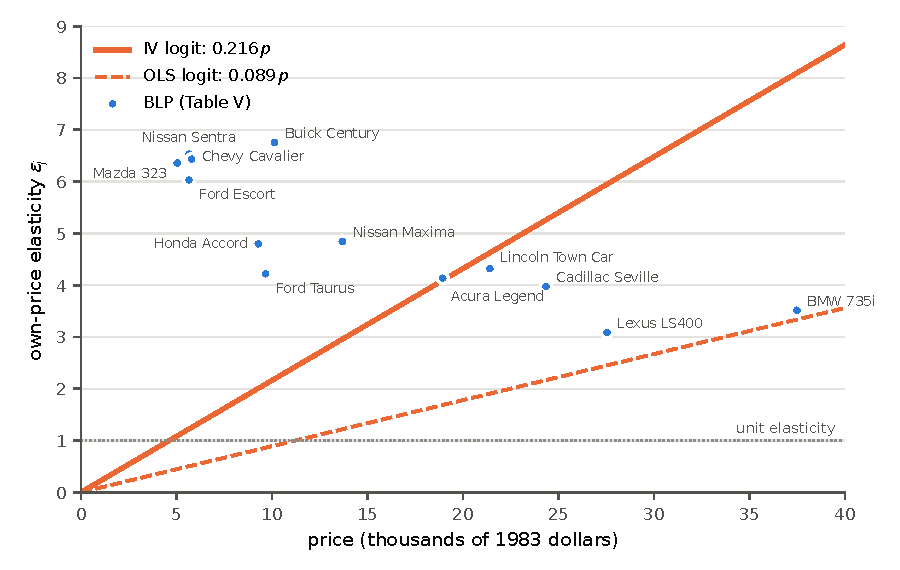
\includegraphics[width=0.86\textwidth]{figures/ch08/blp95_ownelas.pdf}
\caption{Own-price elasticities of thirteen 1990 models against price. Points are BLP's estimates
(their Table V). The rays are the logit elasticities $\alpha p$ implied by the IV and OLS logit price
coefficients of their Table III, ignoring the factor $1-s_j\approx1$. The dotted line marks unit
elasticity. Redrawn from \citet{BerryLevinsohnPakes1995}, Tables III and V.}
\label{fig:08-blp-ownelas}
\end{figure}

The price sensitivity of the marginal buyers can be read off the own semi-elasticities. Combining
\eqref{eq:08-blp-dsown} and \eqref{eq:08-blp-semi},
\begin{equation*}
-\frac{e_{jj}}{100}=\frac{1}{s_j}\int\frac{\alpha}{y_i-p_j}\,s_{ij}(1-s_{ij})\,\dd F(\nu_i)
\approx\E\Big[\frac{\alpha}{y_i-p_j}\,\Big|\,i\text{ buys }j\Big],
\end{equation*}
where the approximation uses $s_{ij}\ll1$. The semi-elasticities in \cref{tab:08-blp-semi} below give
$-\frac{e_{jj}}{100}=1.26$ for the Mazda 323, 0.52 for the Accord and 0.094 for the BMW 735i. Dividing
$\alpha=43.501$ by these numbers gives the harmonic mean of residual income $y_i-p_j$ among buyers. It is
about \$35,000 for the Mazda, \$84,000 for the Accord and \$464,000 for the BMW, in 1983 dollars (our
calculation). The specification can make luxury-car demand inelastic enough only by placing its buyers
far in the upper tail of the lognormal income distribution. This is one motivation for adding data on
buyers' incomes, as \citet{BerryLevinsohnPakes2004} and \citet{Petrin2002} later did
(\cref{sec:08-micro,sec:08-blp04}).

\casehead{Cross-price semi-elasticities}
BLP's Table VI reports own- and cross-price semi-elasticities for the same thirteen models.
\Cref{fig:08-blp-semielas} displays the full matrix, and \cref{tab:08-blp-semi} reproduces two diagonal
blocks. Entry $(i,j)$ is the percentage change in the share of row car $i$ when the price of column car
$j$ rises by \$1,000.

\begin{figure}[htbp]
\centering
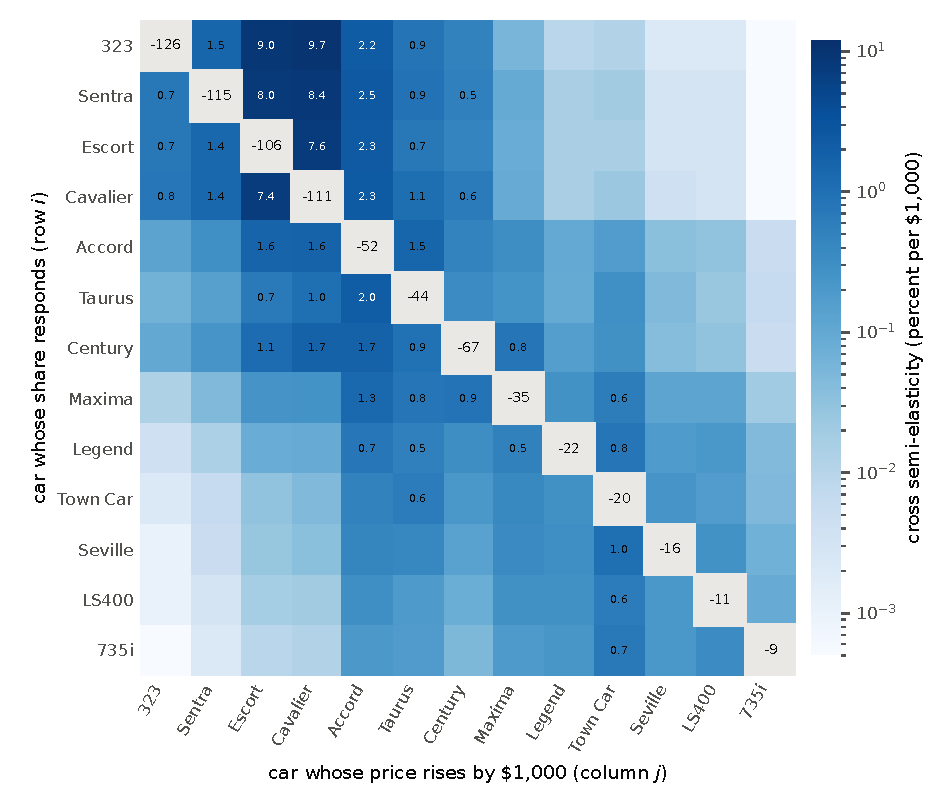
\includegraphics[width=0.9\textwidth]{figures/ch08/blp95_semielas.pdf}
\caption{Own- and cross-price semi-elasticities for thirteen 1990 models. Cell $(i,j)$ is the
percentage change in the share of row car $i$ for a \$1,000 increase in the price of column car $j$.
Off-diagonal cells are shaded on a log scale, and entries of at least 0.5 are printed. Diagonal cells
(gray) print the own semi-elasticity, which is negative. Entries printed as 0.000 in the source are
shaded at the bottom of the scale. Redrawn from \citet{BerryLevinsohnPakes1995}, Table VI.}
\label{fig:08-blp-semielas}
\end{figure}

\begin{table}[htbp]
\centering
\caption{Own- and cross-price semi-elasticities, two blocks of BLP (1995) Table VI}
\label{tab:08-blp-semi}
\small
\begin{tabular}{@{}lrrrr@{}}
\toprule
\multicolumn{5}{@{}l}{\emph{Panel A: small cars}}\\
Share of $\downarrow$ / price of $\rightarrow$ & Mazda 323 & Sentra & Escort & Cavalier \\
\midrule
Mazda 323 & $-125.933$ & 1.518 & 8.954 & 9.680 \\
Sentra    & 0.705 & $-115.319$ & 8.024 & 8.435 \\
Escort    & 0.713 & 1.375 & $-106.497$ & 7.570 \\
Cavalier  & 0.754 & 1.414 & 7.406 & $-110.972$ \\
\midrule
\multicolumn{5}{@{}l}{\emph{Panel B: luxury cars}}\\
Share of $\downarrow$ / price of $\rightarrow$ & Town Car & Seville & LS400 & BMW 735i \\
\midrule
Town Car  & $-20.175$ & 0.226 & 0.168 & 0.048 \\
Seville   & 1.011 & $-16.313$ & 0.263 & 0.068 \\
LS400     & 0.606 & 0.212 & $-11.199$ & 0.086 \\
BMW 735i  & 0.685 & 0.215 & 0.336 & $-9.376$ \\
\midrule
\multicolumn{5}{@{}l}{\emph{Panel C: small-car shares, luxury-car prices}}\\
Share of $\downarrow$ / price of $\rightarrow$ & Town Car & Seville & LS400 & BMW 735i \\
\midrule
Mazda 323 & 0.012 & 0.002 & 0.002 & 0.000 \\
Cavalier  & 0.023 & 0.004 & 0.003 & 0.000 \\
\bottomrule
\end{tabular}

\smallskip
\begin{minipage}{0.86\linewidth}
\footnotesize
Notes: Source: \citet{BerryLevinsohnPakes1995}, Table VI (p.~880), CRTS estimates. Entry
$(i,j)$ is $e_{ij}=\frac{100}{s_i}\frac{\partial s_i}{\partial p_j}$, the percentage change in the
share of row car $i$ for a \$1,000 increase in the price of column car $j$. The full $13\times13$ matrix
is shown in \cref{fig:08-blp-semielas}.
\end{minipage}
\end{table}

Three features stand out. First, own semi-elasticities fall sharply with price, from $-125.9$ for the
Mazda 323 to $-9.4$ for the BMW 735i. Multiplying each by $-\frac{p_j}{100}$ reproduces every own-price
elasticity in \cref{tab:08-blp-attr} to three decimals (our check). Under the IV logit every diagonal
entry would be about $-100\times0.216=-21.6$.

Second, cross effects are large among similar cars and close to zero across segments. A \$1,000 rise in
the Mazda 323's price raises the Sentra's share by 0.705 percent but leaves the Town Car, Seville, Lexus
and BMW almost unaffected. Under the logit the off-diagonal entries of a column would all equal
$100\,\alpha s_j$, whatever the row car. In BLP's matrix the largest cross entry in the Escort column is
about 1,000 times the smallest (8.954 against 0.009).

Third, the closest substitutes are intuitive. Measured down each column, the Lexus is the closest
substitute for the BMW 735i, the Cadillac Seville for the Lincoln Town Car, and the Accord for the Taurus
(p.~881). The effects of a \$1,000 increase are smaller for expensive cars because \$1,000 is a smaller
fraction of their price. Converting to elasticities removes this scale effect. For example, the
elasticity of the Seville's share with respect to the Town Car's price is
$1.011\times\frac{21.412}{100}\approx0.22$.

\casehead{Substitution to the outside good}
BLP measure how much of the demand a car loses goes to the outside good. The statistic is
\begin{equation*}
D_{j0}=100\times\frac{\frac{\partial s_0}{\partial p_j}}{\big|\frac{\partial s_j}{\partial p_j}\big|},
\end{equation*}
the number of consumers who switch from $j$ to no car, as a percentage of all who leave $j$ after a small
price rise. This is the diversion ratio to the outside good. Under the logit,
$\frac{\partial s_0}{\partial p_j}=\alpha s_0s_j$ and
$\big|\frac{\partial s_j}{\partial p_j}\big|=\alpha s_j(1-s_j)$, so
$D_{j0}=100\times\frac{s_0}{1-s_j}$. Under BLP, \cref{prop:08-diversion} gives
\begin{equation*}
\frac{D_{j0}}{100}=\int\varpi_{ij}\,\frac{s_{i0}}{1-s_{ij}}\,\dd F(\nu_i),\qquad
\varpi_{ij}=\frac{\frac{\alpha}{y_i-p_j}\,s_{ij}(1-s_{ij})}
{\int\frac{\alpha}{y_l-p_j}\,s_{lj}(1-s_{lj})\,\dd F(\nu_l)},
\end{equation*}
a weighted average of individual diversions with weights concentrated on the price-sensitive marginal
buyers of $j$.

\begin{table}[htbp]
\centering
\caption{Substitution to the outside good after a price increase (BLP 1995, Table VII)}
\label{tab:08-blp-outside}
\small
\begin{tabular}{@{}lrr@{}}
\toprule
Model & Logit & BLP \\
\midrule
Mazda 323 & 90.870 & 27.123 \\
Nissan Sentra & 90.843 & 26.133 \\
Ford Escort & 90.592 & 27.996 \\
Chevy Cavalier & 90.585 & 26.389 \\
Honda Accord & 90.458 & 21.839 \\
Ford Taurus & 90.566 & 25.214 \\
Buick Century & 90.777 & 25.402 \\
Nissan Maxima & 90.790 & 21.738 \\
Acura Legend & 90.838 & 20.786 \\
Lincoln Town Car & 90.739 & 20.309 \\
Cadillac Seville & 90.860 & 16.734 \\
Lexus LS400 & 90.851 & 10.090 \\
BMW 735i & 90.883 & 10.101 \\
\bottomrule
\end{tabular}

\smallskip
\begin{minipage}{0.62\linewidth}
\footnotesize
Notes: Source: \citet{BerryLevinsohnPakes1995}, Table VII (p.~881). Entries are
$D_{j0}=100\times\frac{\partial s_0}{\partial p_j}\Big(\Big|\frac{\partial s_j}{\partial p_j}\Big|\Big)^{-1}$,
the percentage of consumers who leave car $j$ after a small price increase and choose the outside good.
\end{minipage}
\end{table}

\begin{figure}[htbp]
\centering
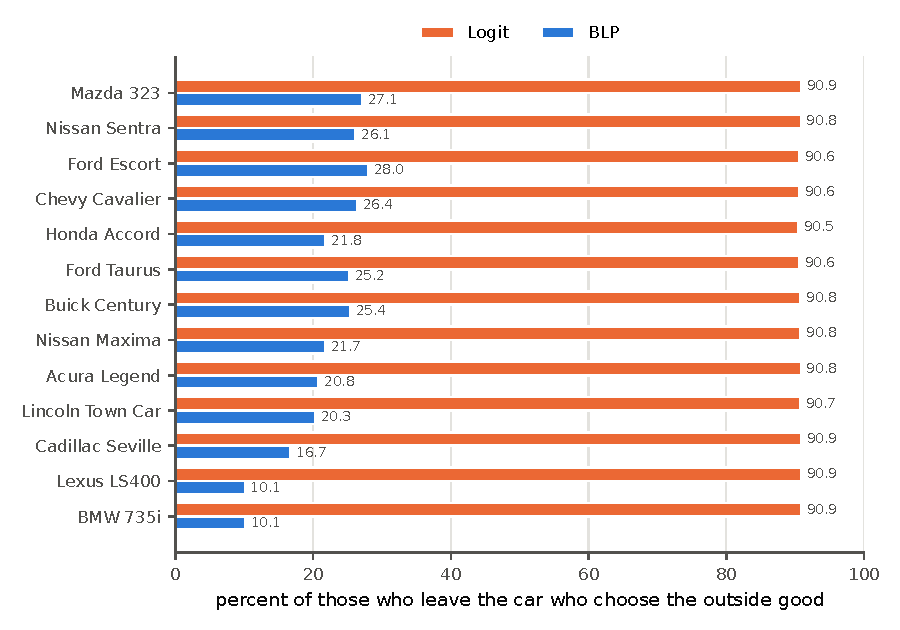
\includegraphics[width=0.82\textwidth]{figures/ch08/blp95_outside.pdf}
\caption{Diversion to the outside good after a small price increase, logit against BLP. Redrawn from
\citet{BerryLevinsohnPakes1995}, Table VII.}
\label{fig:08-blp-outside}
\end{figure}

\Cref{tab:08-blp-outside} and \cref{fig:08-blp-outside} report the results. Under the logit about 90
percent of those who leave any model choose no car, which is $\frac{s_0}{1-s_j}\approx s_0$. The logit
column ranges from 90.458 to 90.883. Since $\frac{s_0}{1-s_j} > s_0$, this puts $s_0$ just below 0.905.
The entries fall slightly with sales, which $\frac{s_0}{1-s_j}$ does not allow, so the printed values
match the formula only approximately. Under
BLP's estimates the diversion ranges from 28.0 percent (Escort) to 10.1 percent (Lexus and BMW). It is
lower for expensive cars. Buyers of luxury cars are rich and like cars, so for them $s_{i0}$ is small and
they move to other luxury cars. Buyers of cheap cars are closer to the margin of not buying. BLP still
find their numbers ``a bit large'' and see this as a sign that the treatment of the outside good needs
improvement (pp.~881--882). The outside good includes keeping an old car, and a dynamic model with a
used-car market would treat it more realistically (Section 8.2 of the paper).

\subsection{Results IV: markups and profits}\label{sec:08-blp95-markups}

Markups combine the demand and cost estimates. \Cref{tab:08-blp-markups} reproduces BLP's Table VIII
and adds four columns that we compute from it and from Table V.

\begin{table}[htbp]
\centering
\caption{Markups and variable profits for 1990 models, CRTS estimates (BLP 1995, Table VIII, with
derived columns)}
\label{tab:08-blp-markups}
\footnotesize
\setlength{\tabcolsep}{4pt}
\begin{tabular}{@{}llrrrrrrr@{}}
\toprule
 & & \multicolumn{3}{c}{BLP Table VIII} & \multicolumn{4}{c}{Derived (our calculation)} \\
\cmidrule(lr){3-5}\cmidrule(l){6-9}
Model & Firm & Price & $p-mc$ & $q(p-mc)$ & $\frac{p-mc}{p}$ & $\frac{1}{\varepsilon_j}$ & Gap
 & Sales \\
\midrule
Mazda 323        & Mazda  & 5,049  & 801    & 18,407  & 0.159 & 0.157 & 0.001 & 22,980 \\
Nissan Sentra    & Nissan & 5,661  & 880    & 43,554  & 0.155 & 0.153 & 0.002 & 49,493 \\
Ford Escort      & Ford   & 5,663  & 1,077  & 311,068 & 0.190 & 0.166 & 0.024 & 288,828 \\
Chevy Cavalier   & GM     & 5,797  & 1,302  & 384,263 & 0.225 & 0.155 & 0.069 & 295,133 \\
Honda Accord     & Honda  & 9,292  & 1,992  & 830,842 & 0.214 & 0.208 & 0.006 & 417,089 \\
Ford Taurus      & Ford   & 9,671  & 2,577  & 807,212 & 0.266 & 0.237 & 0.029 & 313,237 \\
Buick Century    & GM     & 10,138 & 2,420  & 271,446 & 0.239 & 0.148 & 0.091 & 112,168 \\
Nissan Maxima    & Nissan & 13,695 & 2,881  & 288,291 & 0.210 & 0.206 & 0.004 & 100,066 \\
Acura Legend     & Honda  & 18,944 & 4,671  & 250,695 & 0.247 & 0.242 & 0.005 & 53,671 \\
Lincoln Town Car & Ford   & 21,412 & 5,596  & 832,082 & 0.261 & 0.231 & 0.030 & 148,692 \\
Cadillac Seville & GM     & 24,353 & 7,500  & 249,195 & 0.308 & 0.252 & 0.056 & 33,226 \\
Lexus LS400      & Toyota & 27,544 & 9,030  & 371,123 & 0.328 & 0.324 & 0.004 & 41,099 \\
BMW 735i         & BMW    & 37,490 & 10,975 & 114,802 & 0.293 & 0.284 & 0.008 & 10,460 \\
\bottomrule
\end{tabular}

\smallskip
\begin{minipage}{0.97\linewidth}
\footnotesize
Notes: Columns 3 to 5 are from \citet{BerryLevinsohnPakes1995}, Table VIII (p.~882), whose
caption refers to ``Table 6 (CRTS)'' estimates, meaning those of Table IV. Price and markup are in 1983
dollars, and variable profits in thousands of 1983 dollars. ``Firm'' is the parent company. The last
four columns are our calculations: the Lerner index, the inverse own-price elasticity from Table V, the
gap between them, and implied unit sales $\frac{q(p-mc)}{p-mc}$.
\end{minipage}
\end{table}

\casehead{Levels and pattern}
In 1990 the average markup is \$3,753 and the average ratio of markup to price is 0.239 (p.~882). The
lowest markups are those of the Mazda 323 (\$801), Sentra (\$880) and Escort (\$1,077). The Lexus and
BMW have markups of \$9,030 and \$10,975. Markups rise almost monotonically with price, and the Lerner
index rises from about 0.16 to about 0.3. \Cref{fig:08-blp-markup} contrasts this pattern with the IV
logit, whose markups all lie in a band between \$4,630 and \$4,805. BLP note that the average level of
markups is similar in the two models even though the pattern differs (footnote 31).

\begin{figure}[htbp]
\centering
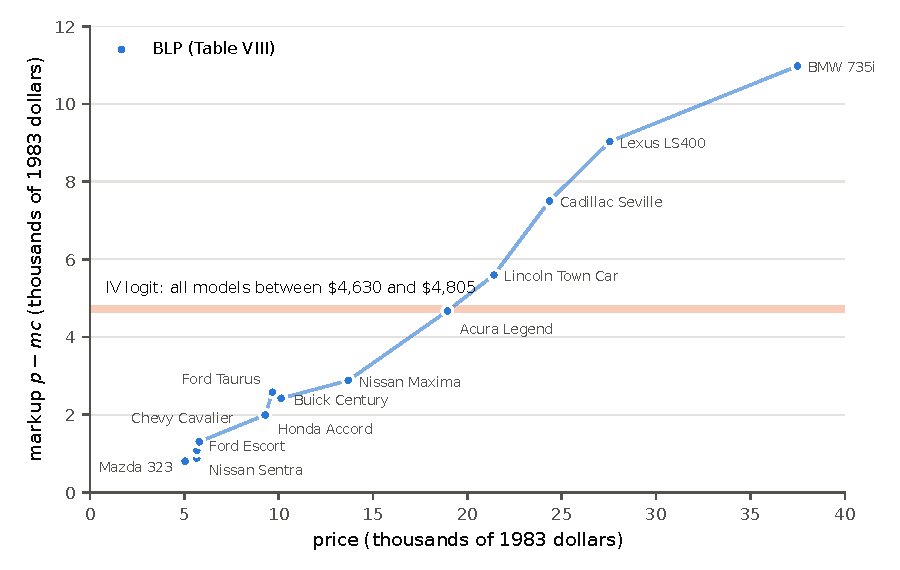
\includegraphics[width=0.86\textwidth]{figures/ch08/blp95_markup.pdf}
\caption{Price-cost markups of thirteen 1990 models against price. Points are BLP's estimates (their
Table VIII). The shaded band is the range of markups implied by the IV logit for all 1990 models
(\$4,630 to \$4,805, p.~874). Redrawn from \citet{BerryLevinsohnPakes1995}.}
\label{fig:08-blp-markup}
\end{figure}

\casehead{Profits}
Large markups need not mean large profits, because some high-markup cars sell few units. BLP single out
the Honda Accord and the Ford Taurus as the most profitable models in their table, by a factor of two
relative to most others. Both were regarded as essential to their firms' finances
(p.~882).\footnote{In the printed Table VIII the Lincoln Town Car's variable profit (\$832,082 thousand)
is as large as the Accord's (\$830,842 thousand) and the Taurus's (\$807,212 thousand). The text's
statement fits the other ten models.} Dividing variable profits by markups recovers unit sales, which
range from 10,460 BMW 735i's to 417,089 Accords.

\casehead{Multi-product pricing in the markups}
The derived columns of \cref{tab:08-blp-markups} reveal the role of multi-product ownership. The
following decomposition holds in any Bertrand-Nash equilibrium.

\begin{proposition}[Multi-product Lerner index]\label{prop:08-blp-lerner}
Let $D_{jr}=\frac{\partial s_r}{\partial p_j}\Big(\Big|\frac{\partial s_j}{\partial p_j}\Big|\Big)^{-1}$
be the diversion ratio from $j$ to $r$. At an interior Bertrand-Nash equilibrium, every product $j$ of firm $f$ satisfies
\begin{equation*}
\frac{p_j-mc_j}{p_j}=\frac{1}{\varepsilon_j}
 +\sum_{r\in\mathcal{J}_f,\,r\neq j}D_{jr}\,\frac{p_r-mc_r}{p_j}.
\end{equation*}
If the products are substitutes and markups are positive, the second term is nonnegative, so
$\varepsilon_j>1$ whenever the Lerner index is below one.
\end{proposition}

\begin{proof}
Move the own-product term of \eqref{eq:08-foc} to the left:
\begin{equation*}
(p_j-mc_j)\Big(-\frac{\partial s_j}{\partial p_j}\Big)=s_j
 +\sum_{r\in\mathcal{J}_f,\,r\neq j}(p_r-mc_r)\frac{\partial s_r}{\partial p_j}.
\end{equation*}
Divide both sides by $p_j\big|\frac{\partial s_j}{\partial p_j}\big|$. The first term on the right
becomes $\frac{s_j}{p_j}\Big(\Big|\frac{\partial s_j}{\partial p_j}\Big|\Big)^{-1}=\frac{1}{\varepsilon_j}$,
and each term of the
sum becomes $D_{jr}\frac{p_r-mc_r}{p_j}$. With substitutes $D_{jr}\geq0$ and positive markups, so the
sum is nonnegative. Then $\frac{1}{\varepsilon_j}\leq\frac{p_j-mc_j}{p_j}<1$ gives
$\varepsilon_j>1$.
\end{proof}

The gap between the Lerner index and $\frac{1}{\varepsilon_j}$ measures the margins a firm recaptures
on its other products. For the products of Mazda, Nissan, Honda, Toyota and BMW the gap is at most
0.008. Their 1990 portfolios contained few close substitutes for these models. For Ford's Escort, Taurus
and Town Car the gap is 0.024 to 0.030. For GM's Cavalier, Century and Seville it is 0.056 to 0.091.
GM's many divisions sell close substitutes for each of its models, so a price rise on the Century
diverts many buyers to other GM cars. This portfolio effect, invisible in the logit except through
$S_f$, is the mechanism that \citet{Nevo2001} later used to separate multi-product pricing from collusion
(\cref{sec:08-nevo01}).

\subsection{Robustness}\label{sec:08-blp95-robust}

The choice of characteristics in utility and cost is ad hoc, and computation limits the number of
random coefficients. BLP report how markups change across six alternative specifications. They choose
markups as the summary because markups combine demand and cost information and are easy to interpret.
\Cref{tab:08-blp-robust} reproduces their Table IX.

\begin{table}[htbp]
\centering
\caption{Markups under alternative specifications, 1990 models, dollars (BLP 1995, Table IX)}
\label{tab:08-blp-robust}
\footnotesize
\setlength{\tabcolsep}{4pt}
\begin{tabular}{@{}lrrrrrrr@{}}
\toprule
 & (1) & (2) & (3) & (4) & (5) & (6) & (7) \\
 & \makecell{Base\\(Table VIII)} & \makecell{$\ln q$\\in cost} & \makecell{AT\\for Air}
 & \makecell{Weight, HP\\for HPWT} & \makecell{Cost\\interactions} & \makecell{Regions,\\reliability}
 & \makecell{Weight,\\interactions} \\
\midrule
Mazda 323        & 801    & 1,616  & 1,012 & 1,073 & 828    & 1,125  & 1,389 \\
Nissan Sentra    & 880    & 1,769  & 1,153 & 1,271 & 912    & 1,308  & 1,487 \\
Ford Escort      & 1,077  & 2,043  & 1,326 & 1,470 & 1,111  & 2,094  & 1,690 \\
Chevy Cavalier   & 1,302  & 2,490  & 1,729 & 1,655 & 1,329  & 2,593  & 2,020 \\
Honda Accord     & 1,992  & 3,059  & 2,629 & 2,703 & 2,059  & 3,839  & 2,327 \\
Ford Taurus      & 2,577  & 3,721  & 2,528 & 3,344 & 2,585  & 4,094  & 2,898 \\
Buick Century    & 2,420  & 4,162  & 3,161 & 2,939 & 2,405  & 4,030  & 3,321 \\
Nissan Maxima    & 2,881  & 4,674  & 4,565 & 2,085 & 2,911  & 6,941  & 3,513 \\
Acura Legend     & 4,671  & 7,105  & 6,563 & 3,059 & 4,661  & 8,305  & 5,081 \\
Lincoln Town Car & 5,596  & 8,029  & 6,778 & 4,765 & 5,508  & 7,114  & 6,518 \\
Cadillac Seville & 7,500  & 10,733 & 8,635 & 4,863 & 7,439  & 9,182  & 8,015 \\
Lexus LS400      & 9,030  & 10,510 & 8,411 & 4,791 & 8,585  & 10,925 & 7,398 \\
BMW 735i         & 10,975 & 13,646 & 9,122 & 7,605 & 10,713 & 12,153 & 12,202 \\
\midrule
Demand variables significant & 5 of 5 & 4 of 5 & 4 of 5 & 6 of 6 & 4 of 5 & 8 of 8 & 4 of 6 \\
\bottomrule
\end{tabular}

\smallskip
\begin{minipage}{0.97\linewidth}
\footnotesize
Notes: Source: \citet{BerryLevinsohnPakes1995}, Table IX (p.~883). Price minus marginal cost in
1983 dollars. (2) adds $\ln q$ to the cost function (last columns of Table IV). (3) replaces Air with a
dummy for standard automatic transmission. (4) replaces HPWT with horsepower and weight entered
separately. (5) adds interactions of the continuous characteristics to the cost function. (6) replaces
the constant in utility with U.S., Japan and Europe dummies and adds the reliability rating. (7) adds
weight and cost-side interactions. The last row counts demand variables whose mean or standard
deviation is significant at the 95 percent level.
\end{minipage}
\end{table}

The pattern of markups survives every specification. In each column markups rise broadly with price, with a few
reversals, and the correlation of each column with the base column is between 0.945 and 0.9997 (our calculation). Levels
move more. Across the seven columns a car's highest markup is between 1.6 and 3.3 times its lowest.

The individual columns have specific explanations (pp.~883--885). Adding $\ln q$ in column (2) raises
every markup, and it gives the highest markups of all the alternatives, yet even these are not
extraordinarily high. As shown above, its markups over average variable cost are implausible. Using
automatic transmission as the luxury proxy in column (3) raises markups slightly for cheap cars and lowers
them slightly for expensive ones. Entering horsepower and weight separately in column (4) changes markups
the most. It gives implausibly low markups for expensive cars, possibly because cost is not linear in
horsepower and weight. Cost interactions in column (5) leave markups within a few percent of the base,
although most interaction terms are significant. Region dummies with reliability in column (6) raise
markups for several mid-priced models from different regions, for reasons BLP could not identify.
Reliability is included there because region dummies may be correlated with reliability, which would
otherwise sit in $\xi$ and invalidate the instruments. Column (7) adds weight, which has an
insignificant cost coefficient and a significant demand mean, and leaves markups close to the base.

\subsection{Interpretation}\label{sec:08-blp95-interp}

BLP read Tables IV to VIII as evidence that flexible utility gives a more realistic picture of
equilibrium in the industry. Three lessons stand out.

First, instrumenting for price matters even in the logit. It more than doubles the price coefficient
and removes almost all inelastic demands (\cref{tab:08-blp-logit}). Second, random coefficients and
income effects change the economics, beyond the econometrics. Own elasticities fall with price,
substitution runs between similar cars, and diversion to the outside good falls from about 90 percent to
10 to 28 percent. Each of these patterns is impossible in the logit. Third, the implied markups are
plausible in level and pattern. They are consistent with standard multi-product pricing, in which GM's
broad portfolio raises its margins above the inverse elasticity.

The results have clear implications for counterfactuals. A merger simulation built on the logit would
predict uniform markups and diversion mostly to the outside good. It would therefore understate the
price effects of merging close substitutes (\cref{ch:mergers}). A tariff analysis would mispredict which
domestic cars gain from higher import prices. A welfare calculation for a new model would depend on how
much demand it takes from similar cars.

\subsection{Limitations and critiques}\label{sec:08-blp95-critique}

\casehead{Data}
Prices are list prices of base models, so discounts and options are missing. Fleet sales are ignored.
Output is poorly measured for imported models, which limits the cost function. Market size is the number
of households, and every household is assumed to consider buying one new car each year.

\casehead{Exogenous characteristics}
The moment condition \eqref{eq:08-blp-moments} treats observed characteristics as mean independent of
$\xi$ and $\omega$. Firms choose characteristics, and they may choose them knowing $\xi$, so the
instruments may be invalid. BLP raise this concern themselves and sketch a Markov alternative
(\cref{sec:08-blp95-estimation}). They also identify obtaining consistent estimates when observed and
unobserved characteristics are correlated as the easier part of the dynamic problem. Endogenizing the
choice of characteristics is the harder part (Section 8.2 of the paper).

\casehead{Statics and the outside good}
Cars are durable. A household's outside option is often its current car, and its timing of purchases
responds to prices and expectations. A static model with an undifferentiated outside good cannot capture
these choices, which may explain why diversion to the outside good still looks large.

\casehead{Conditional counterfactuals}
Policy analysis with the model holds characteristics and the product set fixed. \citet{PakesBerryLevinsohn1993}
used the estimates to predict average MPG after the 1973 gasoline price shock. The model predicted 1974
and 1975 almost exactly, when characteristics changed little. From 1976 on, new small fuel-efficient
models appeared and the predictions became markedly worse (pp.~885--886).

\casehead{Functional form and the supply side}
All heterogeneity in price sensitivity comes from income through $\alpha\ln(y_i-p_j)$, with one income
dispersion parameter for all years. Our harmonic-mean calculation shows how far into the income tail the
model must place luxury-car buyers. The random coefficients are independent normals. Conduct is assumed
to be Bertrand-Nash and is not tested. The constant-returns cost function produces a negative MPG
coefficient, and the alternative with $\ln q$ implies implausible returns to scale.

\casehead{Aggregate data only}
BLP use no data that link households to the cars they buy. Their own conclusion points to consumer
surveys and to plant-level cost data from the Census Longitudinal Research Database (Section 8.2 of the paper).
\citet{BerryLevinsohnPakes2004} and \citet{Petrin2002} later added consumer-level moments for cars
(\cref{sec:08-micro,sec:08-blp04}), and \citet{Goldberg1995} estimated car demand from household data
(\cref{sec:08-goldberg}).

\casehead{Numerical and instrument sensitivity}
Later work re-examined the estimator. \citet[p.~35]{KnittelMetaxoglou2014} used BLP's automobile data and the
synthetic cereal data of \citet{Nevo2000a}. They found that BLP-type estimates and their implications can vary
with the optimization algorithm and starting values.
\citet{DubeFoxSu2012} showed that a loose tolerance in the contraction can produce false convergence
(\cref{sec:08-inversion,sec:08-practice}). \citet[Section~3]{Armstrong2016} showed that the characteristics-based
instruments can lose their power in markets with many products. Equilibrium markups then vary little.
\citet{ReynaertVerboven2014} and \citet[Section~5]{ConlonGortmaker2020} found in Monte Carlo experiments that
approximations to the optimal instruments improve precision.
These critiques concern implementation, and they leave the framework itself intact.

\subsection{Contribution}\label{sec:08-blp95-contrib}

BLP's contribution is a complete template for empirical work on differentiated products with market-level
data. It combines five elements. Utility is defined over characteristics, with random coefficients and
demographic information from outside the sample. Shares are aggregated by simulation. Mean utilities
are recovered by inverting the share equations with a contraction. A GMM estimator built on structural
errors handles price endogeneity, with instruments derived from oligopoly pricing and exchangeability.
A multi-product Nash pricing equation recovers marginal costs and markups without cost data.

The same template now underlies most empirical work on differentiated-products markets. Applications
include voluntary export restraints on Japanese cars \citep{BerryLevinsohnPakes1999}, mergers
\citep[\cref{ch:mergers}]{Nevo2000b}, the welfare gains from new goods
\citep[\cref{ch:newgoods}]{Petrin2002}, and airline hubs \citep[\cref{ch:airlines}]{BerryCarnallSpiller2006}.
\citet{Nevo2000a} wrote the guide that made the method accessible, and we turn to it next.

\section{Case study: Nevo (2000a), the practitioner's guide and its application}\label{sec:08-nevo00}

\citet{Nevo2000a} is a guide to the random coefficients logit for researchers who have not used it. It
explains the model, the algorithm and the instruments with the stated aim of lowering the barriers to
entry and increasing trust in the method among outsiders (p.~514). It ends with an application to a
synthetic data set, and Nevo posted the data and his Matlab code. The model and algorithm of
\cref{sec:08-model,sec:08-substitution,sec:08-simulation,sec:08-inversion,sec:08-gmm,sec:08-instruments}
follow the guide's equations closely. This section covers the rest: the guide's framing, its
specification choices and their implications, its practical advice, the application in full, and its
list of extensions.

\subsection{Purpose and framing}\label{sec:08-nevo00-purpose}

Nevo starts from two problems that make differentiated-products demand hard. The first is
dimensionality. A log-log demand system for 100 products has 100 equations, each with 100 prices, which
means at least 10,000 parameters (p.~514). Symmetry and adding up remove only part of these, and the
number remains too large to estimate. More flexible substitution patterns make the problem worse. The
second is heterogeneity. If all consumers were identical, markets would not show the variety of products
we observe. A representative consumer exists under Gorman-form preferences \citep{Gorman1959}, but those
assumptions are strong and often empirically false.

The logit model solves the dimensionality problem by projecting products onto a space of
characteristics. The number of parameters then depends on the number of characteristics and not on the
square of the number of products. The cost is the logit's treatment of heterogeneity, which makes
substitution depend on market shares and not on how similar products are. Random coefficients keep the
projection and model heterogeneity explicitly. Nevo lists three advantages of the BLP method over earlier
estimates of such models (p.~515). It needs only market-level price and quantity data, it deals with the
endogeneity of prices, and it produces more realistic elasticities.

\subsection{Specification choices and their implications}\label{sec:08-nevo00-spec}

\casehead{The guide's model}
The guide's model is the one of \cref{sec:08-linear}. Indirect utility is \eqref{eq:08-nevo-utility} (his
eq.~1), and tastes depend on demographics and unobserved characteristics as in \eqref{eq:08-tastes} (his
eq.~2). The unobserved tastes $\nu_i$ come from a parametric distribution, usually standard normal, and the
demographics $D_i$ from an empirical distribution such as CPS draws. The outside good is normalized as in \cref{sec:08-normalization}. Combining the
two equations gives the decomposition \eqref{eq:08-decomposition} (his eq.~3), and shares integrate over
$(D,\nu,\epsilon)$ with the factorization \eqref{eq:08-share-bayes} (his eq.~4).

\casehead{Assumptions and their implications}
Nevo spells out three assumptions implicit in \eqref{eq:08-nevo-utility} and then discusses how
\eqref{eq:08-tastes} models heterogeneity (pp.~517--520).
\begin{enumerate}
\item \emph{No wealth effects.} The form $\alpha_i(y_i-p_{jt})$ comes from quasilinear utility. This is
  reasonable for ready-to-eat cereal and unreasonable for cars. BLP's $\ln(y_i-p_j)$ is one alternative,
  and a flexible function $f(y_i-p_{jt})$ is another, as in \citet{Petrin2002}.
\item \emph{A common valuation of $\xi$.} Every consumer values the unobserved characteristic equally.
  Because the price coefficient varies, this is consistent with theories of vertical differentiation.
  \citet{DasOlleyPakes1994} model a distribution of valuations of $\xi$ instead.
\item \emph{Common prices and characteristics.} All consumers in a market face the same price. If they
  do not, a list or average price measures the relevant price with error. This is one more reason why
  price may be correlated with the error. The inversion method handles measurement error only if the
  mismeasured variable enters $\delta_{jt}$ alone (footnote 11, citing \citealp{Berry1994}).
\item \emph{Observed and unobserved heterogeneity.} Demographics bring outside information into the
  model and reduce reliance on parametric assumptions. Nevo's example of an unobserved characteristic is
  whether a household owns a dog, which matters for choosing a car but appears in no survey (p.~519). The
  linear form $\Pi D_i$ is restrictive, especially for the price coefficient.
\end{enumerate}

\casehead{Where correlation in utility comes from}
Nevo then explains why the logit fails and how to fix it (pp.~522--526), with the arguments and the cereal
examples that \cref{sec:08-logit-benchmark} reproduced. The cure is correlation in utility across brands, which
can enter through $\epsilon$ or through $\mu$.
Generalized extreme value models put it in $\epsilon$. The nested logit groups brands into exhaustive and
mutually exclusive nests fixed in advance. Within a nest, substitution is again proportional to shares,
and the model does nothing for own elasticities. \citet{Cardell1997} shows the distributional assumptions
under which a random coefficient on segment dummies reproduces the nested logit. With several layers of
segmentation the order of the nests matters. Grouping computers first by brand and then by technology
gives different substitution than the reverse order, even with the same groups (footnote 18). The
principles-of-differentiation GEV model of \citet{BresnahanSternTrajtenberg1997} avoids ordering the
nests. An unrestricted covariance matrix for $\epsilon$ reintroduces the dimensionality problem.

The random coefficients model puts the correlation in $\mu$. Products with similar characteristics are
correlated in utility, and consumers with similar demographics rank products similarly. The own-price
derivative averages individual price sensitivities with weights given by individual purchase
probabilities (\cref{prop:08-derivs}). If the buyers of Kellogg's Corn Flakes are price sensitive, its
own elasticity is high despite its low price (p.~526). Substitution is then driven by differences in
price sensitivity across the buyers of different products, and not by the functional form.

\subsection{Practical recommendations}\label{sec:08-nevo00-practice}

The guide's Section 3 turns from the model to practice. Most of its advice is now part of the chapter's
theory, and we list each item with the place where we develop it.

\casehead{Data and market size}
The data requirements and Nevo's four rules for choosing the market size are those of \cref{sec:08-data}
(p.~527). Nevo strongly recommends several markets with variation in relative prices or in the products
offered.

\casehead{Two roles of characteristics}
Characteristics explain mean utility $\delta$ and drive substitution through $\mu$, and Nevo recommends keeping
the two roles separate (pp.~527--528, \cref{sec:08-assumptions}). Substitution must come from characteristics,
which should therefore guide what the researcher collects.

\casehead{Identification}
Nevo's informal argument starts from an ideal experiment that randomizes prices across consumers
(pp.~528--530). Market data depart from it in two ways. Prices are set by firms that know $\xi$, which
instruments address. More subtly, a discrete choice model can be estimated from one market. Each market
is then an observation on the relative likelihood of buying $J$ bundles of attributes, one of which is
price. Identification improves with more markets that vary in product characteristics, choice sets and
demographic distributions. His three-product example (A and B similar, B and C with equal shares) appears in
\cref{sec:08-illustration,sec:08-iv-roles}.

\casehead{The estimator}
The guide argues against matching shares by nonlinear least squares (his eq.~7) and builds the GMM residual
from the inverted mean utilities (his eqs.~8 to 13). It notes that the logit and nested logit reduce to
two-stage least squares. \Cref{sec:08-gmm} develops all three points.

\casehead{Instruments}
Nevo reviews cost shifters, characteristics-based instruments and Hausman instruments with their caveats
(pp.~534--536), as in \cref{sec:08-iv-families}. His footnote 23 makes the characteristics-based instruments
concrete. Suppose there are two characteristics (horsepower and size) and two firms with three products each.
The instruments for a product are then its two characteristics, their sums over the firm's other two products,
and their sums over the rival's three products, six in all. Nevo stresses that validity must be argued case by
case.

\casehead{Brand dummies and minimum distance}
Nevo believes brand fixed effects should be used whenever possible (p.~536). \Cref{sec:08-brand-fe} develops his
argument, his answers to the two objections and the minimum-distance estimator \eqref{eq:08-md} of the taste
parameters (pp.~537--538). The assumption $\E[\xi_b\mid \bm{X}_b]=0$ is used only to recover $\beta$. A
researcher unwilling to make it can still recover price sensitivity from the other instruments (footnote 24).

\subsection{The application}\label{sec:08-nevo00-app}

\casehead{Data}
The data contain prices and quantities for 24 brands of a differentiated product in 47 cities over 2
quarters (p.~538). A market is a city-quarter, so there are 94 markets and $24\times94=2{,}256$
observations. Every brand is sold in every market, so choice sets do not vary. The data were generated
from the demand model of Section 2 and a multi-product Bertrand pricing model (footnote 25). The marginal
costs and parameters were motivated by the cereal estimates of \citet{Nevo2000b}. Nevo warns that the data
are not real and should not be used for analysis. Their purpose is to teach the method.

Products have two characteristics. \emph{Sugar} measures sugar content, and \emph{Mushy} equals one if
the cereal gets soggy in milk. Demographics are drawn from the CPS: the log of income (\emph{Income}), its
square (\emph{IncomeSq}), \emph{Age}, and \emph{Child}, a dummy for being under sixteen. The unobserved
$\nu_i$ are standard normal, and each market uses $n_s=20$ simulated individuals. All specifications
include brand and time dummies. Section~4 does not describe the instruments used in the application.

\casehead{Specification}
The pattern of entries in Nevo's Table I reveals the estimated specification. Write $b_i^p=-\alpha_i$
for the price coefficient, which is what the table reports. Then
\begin{align*}
b_i^{p}&=b^{p}+\pi_{p,1}\mathit{Income}_i+\pi_{p,2}\mathit{IncomeSq}_i+\pi_{p,3}\mathit{Child}_i
 +\sigma_p\nu_{ip},\\
\beta_i^{k}&=\beta^{k}+\pi_{k,1}\mathit{Income}_i+\pi_{k,2}\mathit{Age}_i+\sigma_k\nu_{ik},
 \qquad k\in\{\text{Constant},\text{Sugar},\text{Mushy}\}.
\end{align*}
The nonlinear parameters are four standard deviations and nine demographic interactions, so $\theta_2$
has 13 elements. The means of the constant, Sugar and Mushy are absorbed by the brand dummies and
recovered by the minimum-distance step \eqref{eq:08-md} with 24 brand effects.

\begin{table}[htbp]
\centering
\caption{Results from the full model, synthetic cereal data (Nevo 2000a, Table I)}
\label{tab:08-nevo00-results}
\small
\begin{tabular}{@{}lrrrrrr@{}}
\toprule
 & Means & Std.\ dev. & \multicolumn{4}{c}{Interactions with demographic variables} \\
\cmidrule(l){4-7}
Variable & $\beta$ & $\sigma$ & Income & IncomeSq & Age & Child \\
\midrule
Price    & $-32.433$ & 1.848 & 16.598 & $-0.659$ & & 11.625 \\
         & (7.743) & (1.075) & (172.334) & (8.955) & & (5.207) \\
Constant & $-1.841^{a}$ & 0.377 & 3.089 & & 1.186 & \\
         & (0.258) & (0.129) & (1.213) & & (1.016) & \\
Sugar    & $0.148^{a}$ & 0.004 & $-0.193$ & & 0.029 & \\
         & (0.258) & (0.012) & (0.005) & & (0.036) & \\
Mushy    & $0.788^{a}$ & 0.081 & 1.468 & & $-1.514$ & \\
         & (0.013) & (0.205) & (0.697) & & (1.103) & \\
\midrule
GMM objective & & & 14.9 & & & \\
(Degrees of freedom) & & & (7) & & & \\
\bottomrule
\end{tabular}

\smallskip
\begin{minipage}{0.9\linewidth}
\footnotesize
Notes: Source: \citet{Nevo2000a}, Table I (p.~539). Based on 2,256 observations. Except where
noted, parameters are GMM estimates. All regressions include brand and time dummy variables.
Asymptotically robust standard errors in parentheses. $^{a}$Estimates from the minimum-distance
procedure. Blank cells are interactions not included in the specification.
\end{minipage}
\end{table}

\casehead{Results}
\Cref{tab:08-nevo00-results} reproduces Nevo's Table I. The minimum-distance means say that the average
consumer gains utility from more sugar (0.148) and from sogginess (0.788). The standard deviations
capture unobserved heterogeneity. Nevo describes them as insignificant both economically and
statistically, and he expects them to stay statistically insignificant even with more efficient
estimation (footnote 26).\footnote{By the printed standard errors, the standard deviation on the
constant (0.377, with standard error 0.129) has a $t$ ratio near 2.9. The other three standard deviations
are insignificant.}

The demographic interactions have economically large point estimates, although most are imprecise. The
valuation of sogginess falls with age ($-1.514$). Nevo says it also falls with income, while the printed
income interaction is positive (1.468).\footnote{The text on p.~540 states that ``the marginal valuation
of sogginess decreases with age and income.'' The income interaction in Table I is $+1.468$ with standard
error 0.697. We report the table.} \Cref{fig:08-nevo00-dists}(a) shows the implied distribution of the
Mushy coefficient across consumers. Most consumers value sogginess positively, but about 31
percent prefer a crunchy cereal (p.~540). Sugar is valued less by richer consumers, and this interaction
is very precisely estimated ($-0.193$, standard error 0.005).

The mean price coefficient is $-32.433$. Children are less price sensitive. Their price coefficient is
higher by 11.625, which is 36 percent of the mean coefficient and 6.3 times the unobserved standard
deviation $\sigma_p=1.848$ (our calculation). Nevo also reports that above-average-income consumers are
less price sensitive. The income terms are very imprecise, with a standard error of 172.334 on the linear
term. \Cref{fig:08-nevo00-dists}(b) shows the distribution of individual price coefficients. It is not
normal, because it inherits the shape of the empirical distribution of demographics. Its mass lies
between about $-70$ and $-15$, so no consumer has a positive price coefficient, although a linear
specification allows one in principle (p.~540).

\begin{figure}[htbp]
\centering
\begin{subfigure}[t]{0.72\textwidth}
\centering
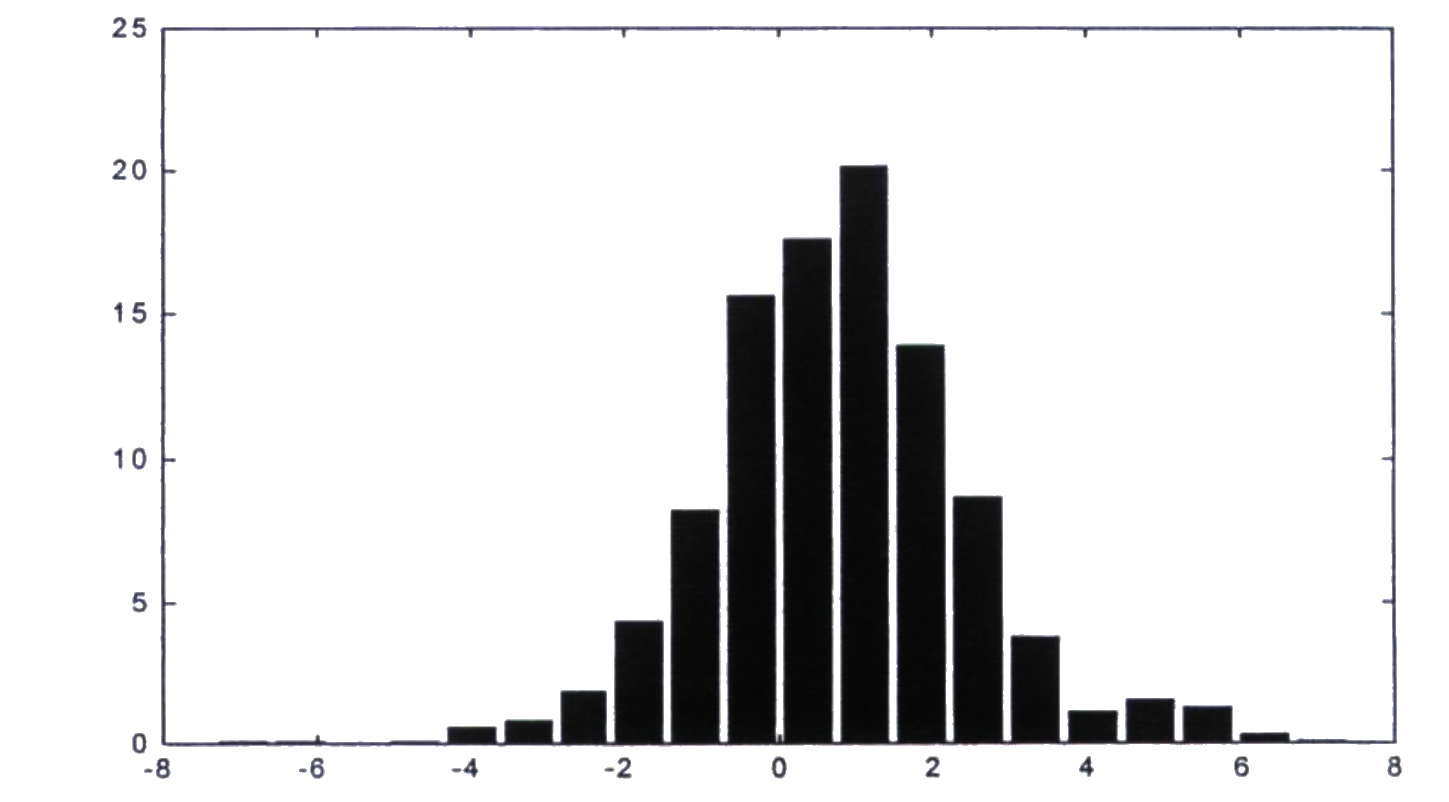
\includegraphics[width=\linewidth]{figures/ch08/nevo00_fig1_mushy.png}
\caption{Taste for sogginess (Mushy coefficient)}
\end{subfigure}

\medskip
\begin{subfigure}[t]{0.72\textwidth}
\centering
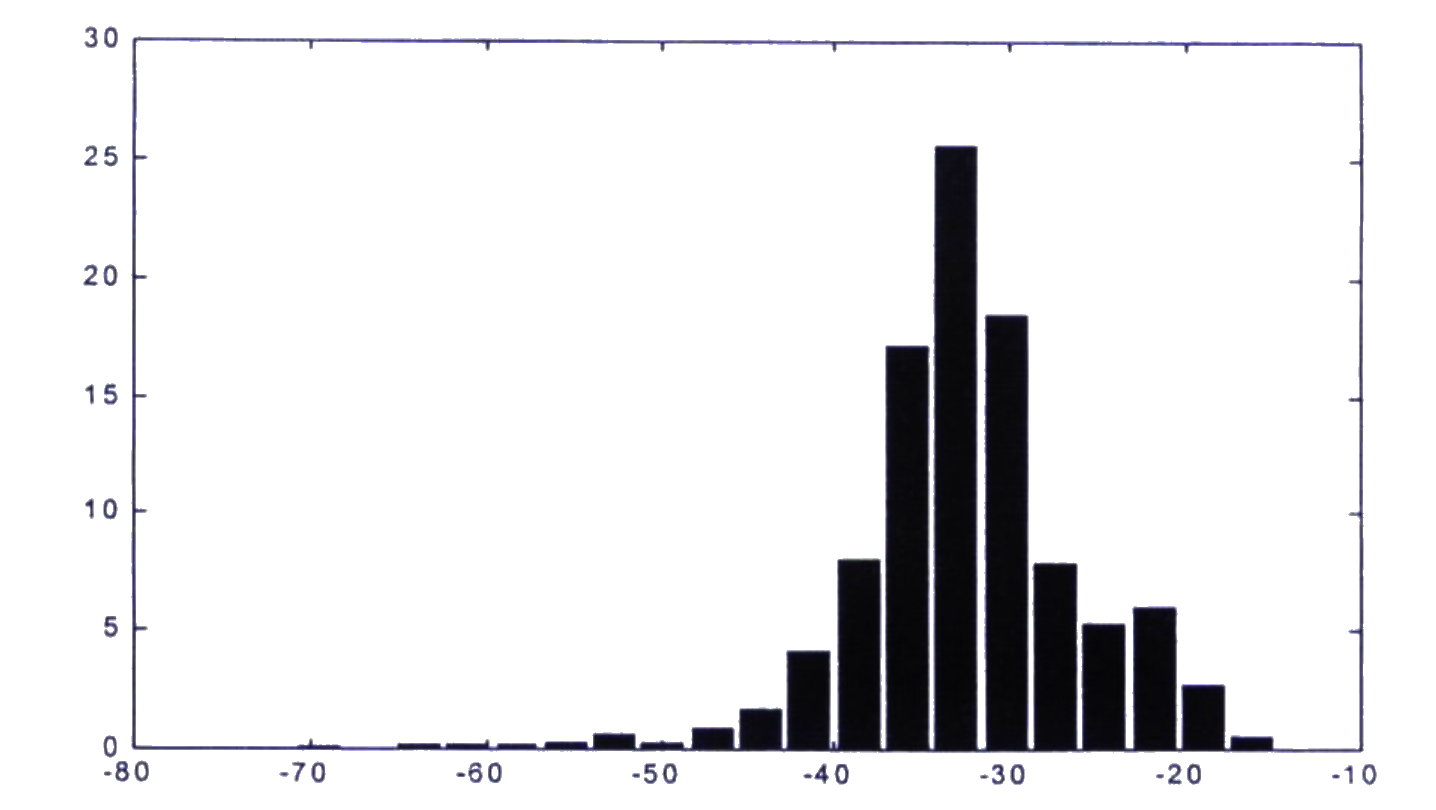
\includegraphics[width=\linewidth]{figures/ch08/nevo00_fig2_price.png}
\caption{Price coefficient}
\end{subfigure}
\caption{Frequency distributions (in percent) of two individual coefficients implied
by the estimates in \cref{tab:08-nevo00-results}. Panel (a) has mass below zero for consumers who prefer
crunchy cereal. Panel (b) is skewed because the empirical distribution of demographics drives it. Source:
\citet{Nevo2000a}, Figures 1 and 2.}
\label{fig:08-nevo00-dists}
\end{figure}

\casehead{Demographics against unobserved tastes}
The standard deviations are small relative to the demographic effects. Nevo computes the share of the
variance of each estimated coefficient explained by demographics, and all these shares exceed 90 percent
(p.~541). He reads this with care. It does not show that demographics explain all heterogeneity. It shows
that the data reject the assumed normal distribution of unobserved tastes. Other work had found that
purchase histories \citep{RossiMcCullochAllenby1996} and second-choice data \citep{BerryLevinsohnPakes2004}
explain heterogeneity beyond demographics (footnote 27). A second explanation is the absence of
choice-set variation across markets in these data, which BLP's data have. Such variation helps identify
the variance of the random shocks (\cref{sec:08-nevo00-practice}). Nevo notes that this explanation
accounts for imprecision, but not for the low point estimates or for the significance of the demographic
effects.

\casehead{Specification tests}
Nevo tests the logit against the full model by testing that all nonlinear parameters are jointly zero,
and the hypothesis is easily rejected (footnote 28). The GMM objective is 14.9 with 7 degrees of freedom.
If the objective is scaled as Hansen's $J$ statistic, this value exceeds the 95th percentile of the
$\chi^2(7)$ distribution, which is 14.07. The $p$-value is about 0.04 (our calculation), a marginal
rejection of the overidentifying restrictions. Nevo does not discuss this statistic.

\casehead{Elasticities}
\Cref{tab:08-nevo00-elas} reproduces Nevo's Table II. It reports the median over the 94 markets of each
own and cross elasticity for nine of the 24 brands, with each brand's characteristics. Entry $(i,j)$ is
the percentage change in the share of row brand $i$ for a one-percent change in the price of column
brand $j$.

\begin{table}[htbp]
\centering
\caption{Median own- and cross-price elasticities, synthetic cereal data (Nevo 2000a, Table II)}
\label{tab:08-nevo00-elas}
\footnotesize
\setlength{\tabcolsep}{3.3pt}
\begin{tabular}{@{}rrrrrrrrrrrr@{}}
\toprule
 & \multicolumn{2}{c}{Characteristics} & \multicolumn{9}{c}{Price of brand} \\
\cmidrule(lr){2-3}\cmidrule(l){4-12}
Brand & Sugar & Mushy & 1 & 2 & 3 & 4 & 5 & 14 & 15 & 19 & 24 \\
\midrule
1  & 2  & 1 & $-2.1689$ & 0.0562 & 0.2429 & 0.1161 & 0.0645 & 0.0596 & 0.0611 & 0.0759 & 0.2375 \\
2  & 18 & 1 & 0.1119 & $-3.4505$ & 0.1302 & 0.0924 & 0.1905 & 0.2305 & 0.2606 & 0.4380 & 0.1165 \\
3  & 4  & 1 & 0.2715 & 0.0674 & $-2.9208$ & 0.1083 & 0.0709 & 0.0627 & 0.0684 & 0.0944 & 0.2237 \\
4  & 3  & 0 & 0.1868 & 0.0736 & 0.1501 & $-3.2709$ & 0.1470 & 0.1557 & 0.1564 & 0.1037 & 0.2670 \\
5  & 12 & 0 & 0.0965 & 0.1540 & 0.0947 & 0.1326 & $-5.5116$ & 0.2852 & 0.3085 & 0.2988 & 0.1715 \\
\addlinespace
6  & 14 & 0 & 0.0699 & 0.1642 & 0.0698 & 0.1123 & 0.2518 & 0.3628 & 0.3971 & 0.3513 & 0.1369 \\
7  & 3  & 1 & 0.2828 & 0.0606 & 0.2390 & 0.1035 & 0.0648 & 0.0563 & 0.0598 & 0.0865 & 0.2225 \\
8  & 4  & 0 & 0.1743 & 0.0789 & 0.1476 & 0.1622 & 0.1524 & 0.1620 & 0.1656 & 0.1180 & 0.2555 \\
9  & 14 & 0 & 0.0735 & 0.1704 & 0.0717 & 0.1128 & 0.2596 & 0.3586 & 0.3966 & 0.3443 & 0.1333 \\
10 & 1  & 0 & 0.2109 & 0.0643 & 0.1682 & 0.1665 & 0.1224 & 0.1199 & 0.1298 & 0.0817 & 0.2809 \\
\addlinespace
11 & 11 & 0 & 0.0967 & 0.1556 & 0.0890 & 0.1377 & 0.2426 & 0.3322 & 0.3427 & 0.2899 & 0.1769 \\
12 & 4  & 1 & 0.2711 & 0.0691 & 0.2339 & 0.1121 & 0.0735 & 0.0662 & 0.0704 & 0.0985 & 0.2260 \\
13 & 3  & 1 & 0.2827 & 0.0597 & 0.2390 & 0.0983 & 0.0632 & 0.0554 & 0.0582 & 0.0866 & 0.2189 \\
14 & 13 & 0 & 0.0834 & 0.1825 & 0.0786 & 0.1247 & 0.2697 & $-3.8393$ & 0.3922 & 0.3380 & 0.1600 \\
15 & 13 & 0 & 0.0889 & 0.1763 & 0.0814 & 0.1256 & 0.2491 & 0.3542 & $-4.3982$ & 0.3383 & 0.1582 \\
\addlinespace
16 & 16 & 1 & 0.1430 & 0.2282 & 0.1523 & 0.0873 & 0.1447 & 0.1442 & 0.1702 & 0.3270 & 0.1264 \\
17 & 10 & 0 & 0.1138 & 0.1399 & 0.1005 & 0.1466 & 0.2172 & 0.2867 & 0.2912 & 0.2498 & 0.1875 \\
18 & 3  & 0 & 0.1900 & 0.0717 & 0.1542 & 0.1656 & 0.1362 & 0.1508 & 0.1578 & 0.1026 & 0.2660 \\
19 & 20 & 1 & 0.0944 & 0.2691 & 0.1130 & 0.0771 & 0.2163 & 0.2618 & 0.3107 & $-3.3335$ & 0.1013 \\
20 & 7  & 0 & 0.1420 & 0.0999 & 0.1270 & 0.1546 & 0.1791 & 0.2074 & 0.2080 & 0.1628 & 0.2251 \\
\addlinespace
21 & 14 & 0 & 0.0773 & 0.1706 & 0.0741 & 0.1160 & 0.2534 & 0.3573 & 0.3794 & 0.3530 & 0.1416 \\
22 & 6  & 0 & 0.1500 & 0.0950 & 0.1283 & 0.1602 & 0.1797 & 0.2096 & 0.2085 & 0.1530 & 0.2311 \\
23 & 12 & 0 & 0.0854 & 0.1561 & 0.0815 & 0.1307 & 0.2559 & 0.3484 & 0.3753 & 0.3154 & 0.1608 \\
24 & 0  & 0 & 0.2249 & 0.0548 & 0.1731 & 0.1619 & 0.1110 & 0.1044 & 0.1114 & 0.0733 & $-4.1215$ \\
\midrule
\multicolumn{3}{@{}l}{Outside good} & 0.0303 & 0.2433 & 0.0396 & 0.0552 & 0.2279 & 0.3349 & 0.3716
 & 0.3896 & 0.0399 \\
\bottomrule
\end{tabular}

\smallskip
\begin{minipage}{0.97\linewidth}
\footnotesize
Notes: Source: \citet{Nevo2000a}, Table II (p.~542). Entry $(i,j)$ is the percentage change in the
market share of row brand $i$ for a one-percent change in the price of column brand $j$. Each entry is the
median over the 94 markets. Only nine of the 24 columns are printed in the source.
\end{minipage}
\end{table}

\casehead{Reading Table II}
Own elasticities among the printed columns range from $-2.17$ (brand 1) to $-5.51$ (brand 5). Cross
elasticities within a column vary with characteristics, unlike the logit, which forces a constant column.
Nevo summarizes this by the ratio of the largest to the smallest cross elasticity in a column, which he
reports varies from 9 to 3 (p.~543).\footnote{Among the nine printed columns, the ratio ranges from 2.2
(brand 4) to 6.8 (brand 15) by our calculation. Nevo's range presumably covers all 24 columns, most of
which are not printed.} A column with a ratio near one shows that the characteristics are too weak to
break the logit pattern for that brand. Nevo suggests the diagnostic can guide which characteristics to
add.

Brands with the same characteristics have nearly identical rows. Nevo points to brands 14 and 15, which
both have Sugar 13 and Mushy 0. The table contains five more such groups: brands 3 and 12, 4 and 18, 5
and 23, 7 and 13, and 6, 9 and 21. The following result explains the pattern.

\begin{proposition}[Products with identical heterogeneous utility]\label{prop:08-nevo00-identical}
Suppose products $j$ and $j'$ have $\mu_{ij}=\mu_{ij'}$ for every consumer $i$. Then for every inside product
$k\notin\{j,j'\}$, the elasticities of $j$ and $j'$ with respect to $p_k$ are equal. Moreover, the diversion from $k$ to $j$ and to $j'$ is in proportion to their shares,
$\frac{D_{kj}}{D_{kj'}}=\frac{s_j}{s_{j'}}$.
\end{proposition}

\begin{proof}
From \eqref{eq:08-individual-share}, $\frac{s_{ij}}{s_{ij'}}=e^{\delta_j-\delta_{j'}}\equiv c$ for every $i$.
Integrating gives $s_j=c\,s_{j'}$, so $\frac{s_{ij}}{s_j}=\frac{s_{ij'}}{s_{j'}}$ for every $i$. The cross
elasticity with respect to $p_k$ is
\begin{equation*}
\varepsilon_{jk}=\frac{p_k}{s_j}\int\alpha_is_{ij}s_{ik}\,\dd F
 =p_k\int\alpha_i\frac{s_{ij}}{s_j}\,s_{ik}\,\dd F ,
\end{equation*}
and the last expression is the same for $j$ and $j'$. For the diversion ratios,
the common denominator $\big|\frac{\partial s_k}{\partial p_k}\big|$ cancels, so
\begin{equation*}
\frac{D_{kj}}{D_{kj'}}=\frac{\int\alpha_is_{ij}s_{ik}\,\dd F}{\int\alpha_is_{ij'}s_{ik}\,\dd F}
 =c=\frac{s_j}{s_{j'}} .
\end{equation*}
\end{proof}

In the application price carries a random coefficient, so $\mu_{ij}$ includes the price term. Two brands
with the same Sugar and Mushy but different prices have slightly different $\mu$. Their rows are
therefore close but not identical, as in brands 14 and 15 (0.0834 against 0.0889 in column 1, 0.2697
against 0.2491 in column 5). The second part of the proposition shows that the random coefficients model
keeps the IIA property among products that differ only in $\xi$. This is the clone problem of
\cref{sec:08-practice}.

The outside-good row varies a lot, from 0.0303 for brand 1 to 0.3896 for brand 19. It rises with the
brand's sugar content. Across the nine printed columns, its correlation with Sugar is 0.90 (our
calculation). Table I suggests why. Richer consumers value inside goods more (the Constant-Income
interaction is 3.089) and value sugar less (the Sugar-Income interaction is $-0.193$). Buyers of sugary
brands are therefore poorer on average, closer to the margin of buying nothing, and they move to the
outside good when prices rise.

\subsection{Lessons, extensions and assessment}\label{sec:08-nevo00-lessons}

\casehead{Lessons from the application}
Nevo stresses economic significance over statistical significance, because most coefficients are
imprecise. He attributes the imprecision to the simplifications made for teaching. More data, more
simulation draws than $n_s=20$, better simulation methods or a supply side would improve efficiency
(p.~540). The application shows four things a user of the method should expect. Demographic interactions
can carry most of the heterogeneity. Distributions of individual coefficients inherit the shape of the
demographic distribution. Elasticity matrices depart clearly from the logit pattern but only as far as
the characteristics allow. Without choice-set variation the standard deviations are hard to pin down.

\casehead{Extensions}
Nevo's Section 5 lists five directions.
\begin{itemize}
\item \emph{Supply side.} In the guide the supply side only motivates the instruments. Specifying it
  adds moment conditions with little extra programming for standard static models (\cref{sec:08-supply}).
  It raises efficiency at the cost of more structure.
\item \emph{Consumer-level data.} With individual choices, models are usually estimated by maximum
  likelihood or simulated moments, as in \citet{Goldberg1995}, \citet{RossiMcCullochAllenby1996} and
  \citet{McFaddenTrain2000}. The mean utilities can be estimated from the micro data and then treated like
  inverted mean utilities, with standard errors that account for their estimation. Endogeneity can
  persist with micro data, because optimal choice from a menu can create it \citep{Kennan1989} and common
  unobserved characteristics remain. Combining micro and aggregate data adds moments, as in
  \citet{Petrin2002} and \citet{BerryLevinsohnPakes2004} (\cref{sec:08-micro,sec:08-blp04,sec:08-goldberg}).
\item \emph{Alternative methods.} Multi-level demand systems use separability to model a category, its
  segments and the brands within each segment, each with a flexible form such as the almost ideal demand
  system \citep{DeatonMuellbauer1980a,HausmanLeonardZona1994}. They become impractical when segments
  contain more than a handful of brands (\cref{ch:aids}).
\item \emph{Dynamics.} The static demand model can feed dynamic models of firm behavior
  \citep{PakesMcGuire1994}, and dynamic models could endogenize characteristics and supply new
  identifying conditions. Demand-side dynamics are better studied with consumer-level data
  \citep{ErdemKeane1996}.
\item \emph{Instruments.} Nevo closes with a warning. Identification rests on adequate exogenous
  instruments, and researchers should not let the technical fireworks distract from this basic and
  difficult problem (p.~546).
\end{itemize}

\casehead{Limitations and critiques}
The application cannot answer any substantive question, because its data are synthetic. Its small number
of draws makes simulation error a real concern (\cref{sec:08-simulation}). The absence of choice-set
variation weakens identification of $\Sigma$, as Nevo notes. The guide's code and data became a standard
test case for later computational work. \citet[Section~6.2]{DubeFoxSu2012} used the cereal data to show how a
loose inner-loop tolerance distorts estimates. They also note that a loose outer-loop tolerance left the guide's
reported estimates short of a local optimum. \citet[p.~39]{KnittelMetaxoglou2014} adapted the
guide's code to study how estimates on these data vary with optimizers and starting values.
\citet[Section~6]{ConlonGortmaker2020} distribute the data with their software and replicate the guide's model on
them. They find that tight optimization tolerances remove this dispersion (\cref{sec:08-practice}).

\casehead{Contribution}
The guide made the method usable. It translated BLP's estimator into explicit steps, explained the role
of each assumption, and gave rules for market size, instruments and brand effects. The posted data and
code let a generation of researchers reproduce every number before applying the method to their own
markets. Its notation, with $\theta_1$, $\theta_2$, $\Pi$ and $\Sigma$, is the notation of this chapter.
Its most durable advice is that heterogeneity should be modeled with outside information wherever possible
and that instruments deserve more attention than computation. \Cref{sec:08-nevo01} turns to Nevo's own
application of the method to market power in ready-to-eat cereal.
